\documentclass[a4paper,12pt]{scrartcl}
%
%Präambel Start
%
%Deutsche Einstellungen Start
\usepackage[ngerman]{babel} 
\usepackage[utf8]{inputenc} %utf-8 eingabe
\usepackage[T1]{fontenc}
\usepackage{pdfpages}
\usepackage{listings}
\usepackage{color}
\usepackage{csquotes}
\usepackage[colorlinks,
pdfpagelabels,
pdfstartview = FitH,
bookmarksopen = true,
bookmarksnumbered = true,
linkcolor = black,
plainpages = false,
hypertexnames = false,
citecolor = black] {hyperref}
\usepackage{fancyhdr}
\usepackage{totpages}
\pagestyle{empty}
\fancyfoot{}
\fancyfoot[R]{\thepage /\ref{TotPages}}
\fancypagestyle{plain}{}
%Quellcodeformatierung
\definecolor{middlegray}{rgb}{0.5,0.5,0.5}
\definecolor{lightgray}{rgb}{0.8,0.8,0.8}
\definecolor{orange}{rgb}{0.8,0.3,0.3}
\definecolor{yac}{rgb}{0.6,0.6,0.1}
\lstset{
	extendedchars=true,
	basicstyle=\scriptsize\ttfamily,
	keywordstyle=\bfseries\ttfamily\color{orange},
	stringstyle=\color{green}\ttfamily,
	commentstyle=\color{middlegray}\ttfamily,
	emph={square}, 
	emphstyle=\color{blue}\texttt,
	emph={[2]root,base},
	emphstyle={[2]\color{yac}\texttt},
	showstringspaces=false,
	flexiblecolumns=false,
	tabsize=2,
	numbers=left,
	numberstyle=\tiny,
	numberblanklines=false,
	stepnumber=1,
	numbersep=10pt,
	xleftmargin=15pt
}
%Ende Quellcodeformatierung
% Deutsche Einstellungen End
%
\title{PROG2 SoSe 2020\\Chaos Reborn Reborn\\Entwicklungsarbeit}
\author{Henning Kröger - 5093186 \\Joshua Christ - 5096129 \\Christian Vicky Temfac Djoken - 5103696\\ Jakob Spohler - 5094026}
\date{\today}
%Präambel End
%
%Inhalt Start
\begin{document}
	\maketitle % erzeugt einen Titel aus title, author und date
	\thispagestyle{empty}
	\newpage % der weitere text wird auf einer neuen seite gedruckt
	\pagestyle{plain}
	\tableofcontents % erzeugt aus sections und subsections ein inhaltsverzeichnis kann auch am ende stehen
	\newpage
	%
	\section{Aufgabenstellung}
	\glqq Sie sollen die Mechanik (Law-Modus) des Spiels Chaos Reborn (http://www.chaos-reborn.com/) in Java nach den unten genannten Anforderungen implementieren und visualisieren, dabei sollen Sie kreativ sein. Beachten Sie, dass Sie nur die unten genannten Anforderungen umsetzen müssen und im 2D bleiben.\grqq \\Quelle: PROG2 SoSe 20 Aufgabe.pdf
	\section{Anforderungsdefinition}
	\begin{enumerate}
		\item Spieler 1 spielt gegen Spieler 2 am selben PC oder über Netzwerk. Das Ziel ist die Auslöschung des anderen Spielers. Jeder Spieler hat einen Wert für Angriff, Verteidigung, Bewegungsradius, Mana und Lebenspunkte.
		
		\item Das Spiel ist rundenbasiert. Es soll \textbf{keine} KI implementiert werden.
		
		\item Es wird auf einer 2D Schachbrett-Karte gespielt. Für die Karten gibt es die Größen Klein, Mittel und Groß.
		
		\item Auf der Karte können Hindernisse sein. Felder mit Hindernissen können nicht betreten werden.
		
		\item Es gibt Manaquellen, die die Spieler beim Betreten des Feldes einmalig mit Mana versorgen. Die Positionen dieser Manaquellen und deren Anzahl wird zufällig bestimmt.
		
		\item Es gibt Erhöhungen der Felder (bis 2 Ebenen). Manche Wesen können solche Erhöhungen nicht betreten. Visualisieren Sie diese Erhöhungen geeignet. So könnten diese mit Grauwerten dargestellt werden, wobei Schwarz ein Hindernis darstellt.
		
		\item Jeder Spieler besitzt ein Deck von Karten. Karten können neutral, chaotisch oder rechtschaffen sein.
		
		\item Mit dem Ausspielen einer Karte wird ein Wesen erschaffen oder ein Zauber ausgelöst.Das Ausspielen einer Karte kostet eine von der Karte bestimmte Menge Mana.
		
		\item Übernehmen Sie die Wesen und Zauber aus Chaos Reborn oder denken Sie sich neue aus.
		
		\item Die Spieler werden zu Beginn des Spiels mit einem zufälligen Zauberstab ausgerüstet. Diese Zauberstäbe bestimmen die Art des Decks, die Anzahl der Karten auf der Hand, den Verbrauch von Mana und wenn sie wollen noch mehr.
		
		\item Es gibt eine Mana-Flux-Anzeige, die zu Beginn des Spiels neutral ist. Die Anzeige verändert sich in die entsprechende Richtung der ausgespielten Karte. Wird eine chaotische Karte gespielt, dann wird die Anzeige in Richtung chaotisch verändert und damit kosten chaotische Karten weniger Mana. Überlegen Sie sich hier eine gute Balance, die auch von Zauberstäben verändert werden kann.
		
		\item Spieler und Wesen können sich pro Runde um eine bestimmte Anzahl von Feldern bewegen und angreifen. Manche Wesen haben Spezialangriffe. Denken Sie bei der Bewegung an Hindernisse und Erhöhungen. Manche Wesen können fliegen.
		
		\item Wesen haben zumindest Lebenspunkte, Angriffswert, Verteidigungswert und Bewegungsradius.
		
		\item Die Spieler und die Wesen werden mit 2D-Bildern auf der Karte dargestellt.
		
		\item Setzen Sie Sound geeignet ein und visualisieren Sie die auf der Karte stattfindenden Aktionen (Selektion, Angriff, Bewegung, usw.) geeignet.
	\end{enumerate}
	\section{Entwurf}
	Um die Anforderungen umzusetzen und das Spiel zu implementieren haben wir einen Entwurf erarbeitet indem wir uns bei einem Brainstorming überlegt haben welche Klassen wir brauchen, welche Attribute diese benötigen und ob wir mit Quadraten oder Hexagonen arbeiten möchten. Wir haben uns für Hexagone entschieden und aus unseren Ergebnissen vom Brainstorming ein UML-Diagramm erstellt dass wir laufend überarbeitet haben.\\ Das Diagramm enthält nur den Teil des Quellcodes in dem wir das Spiel und seine Anforderungen modellieren und ist zoombar ohne unleserlich zu werden.\\
	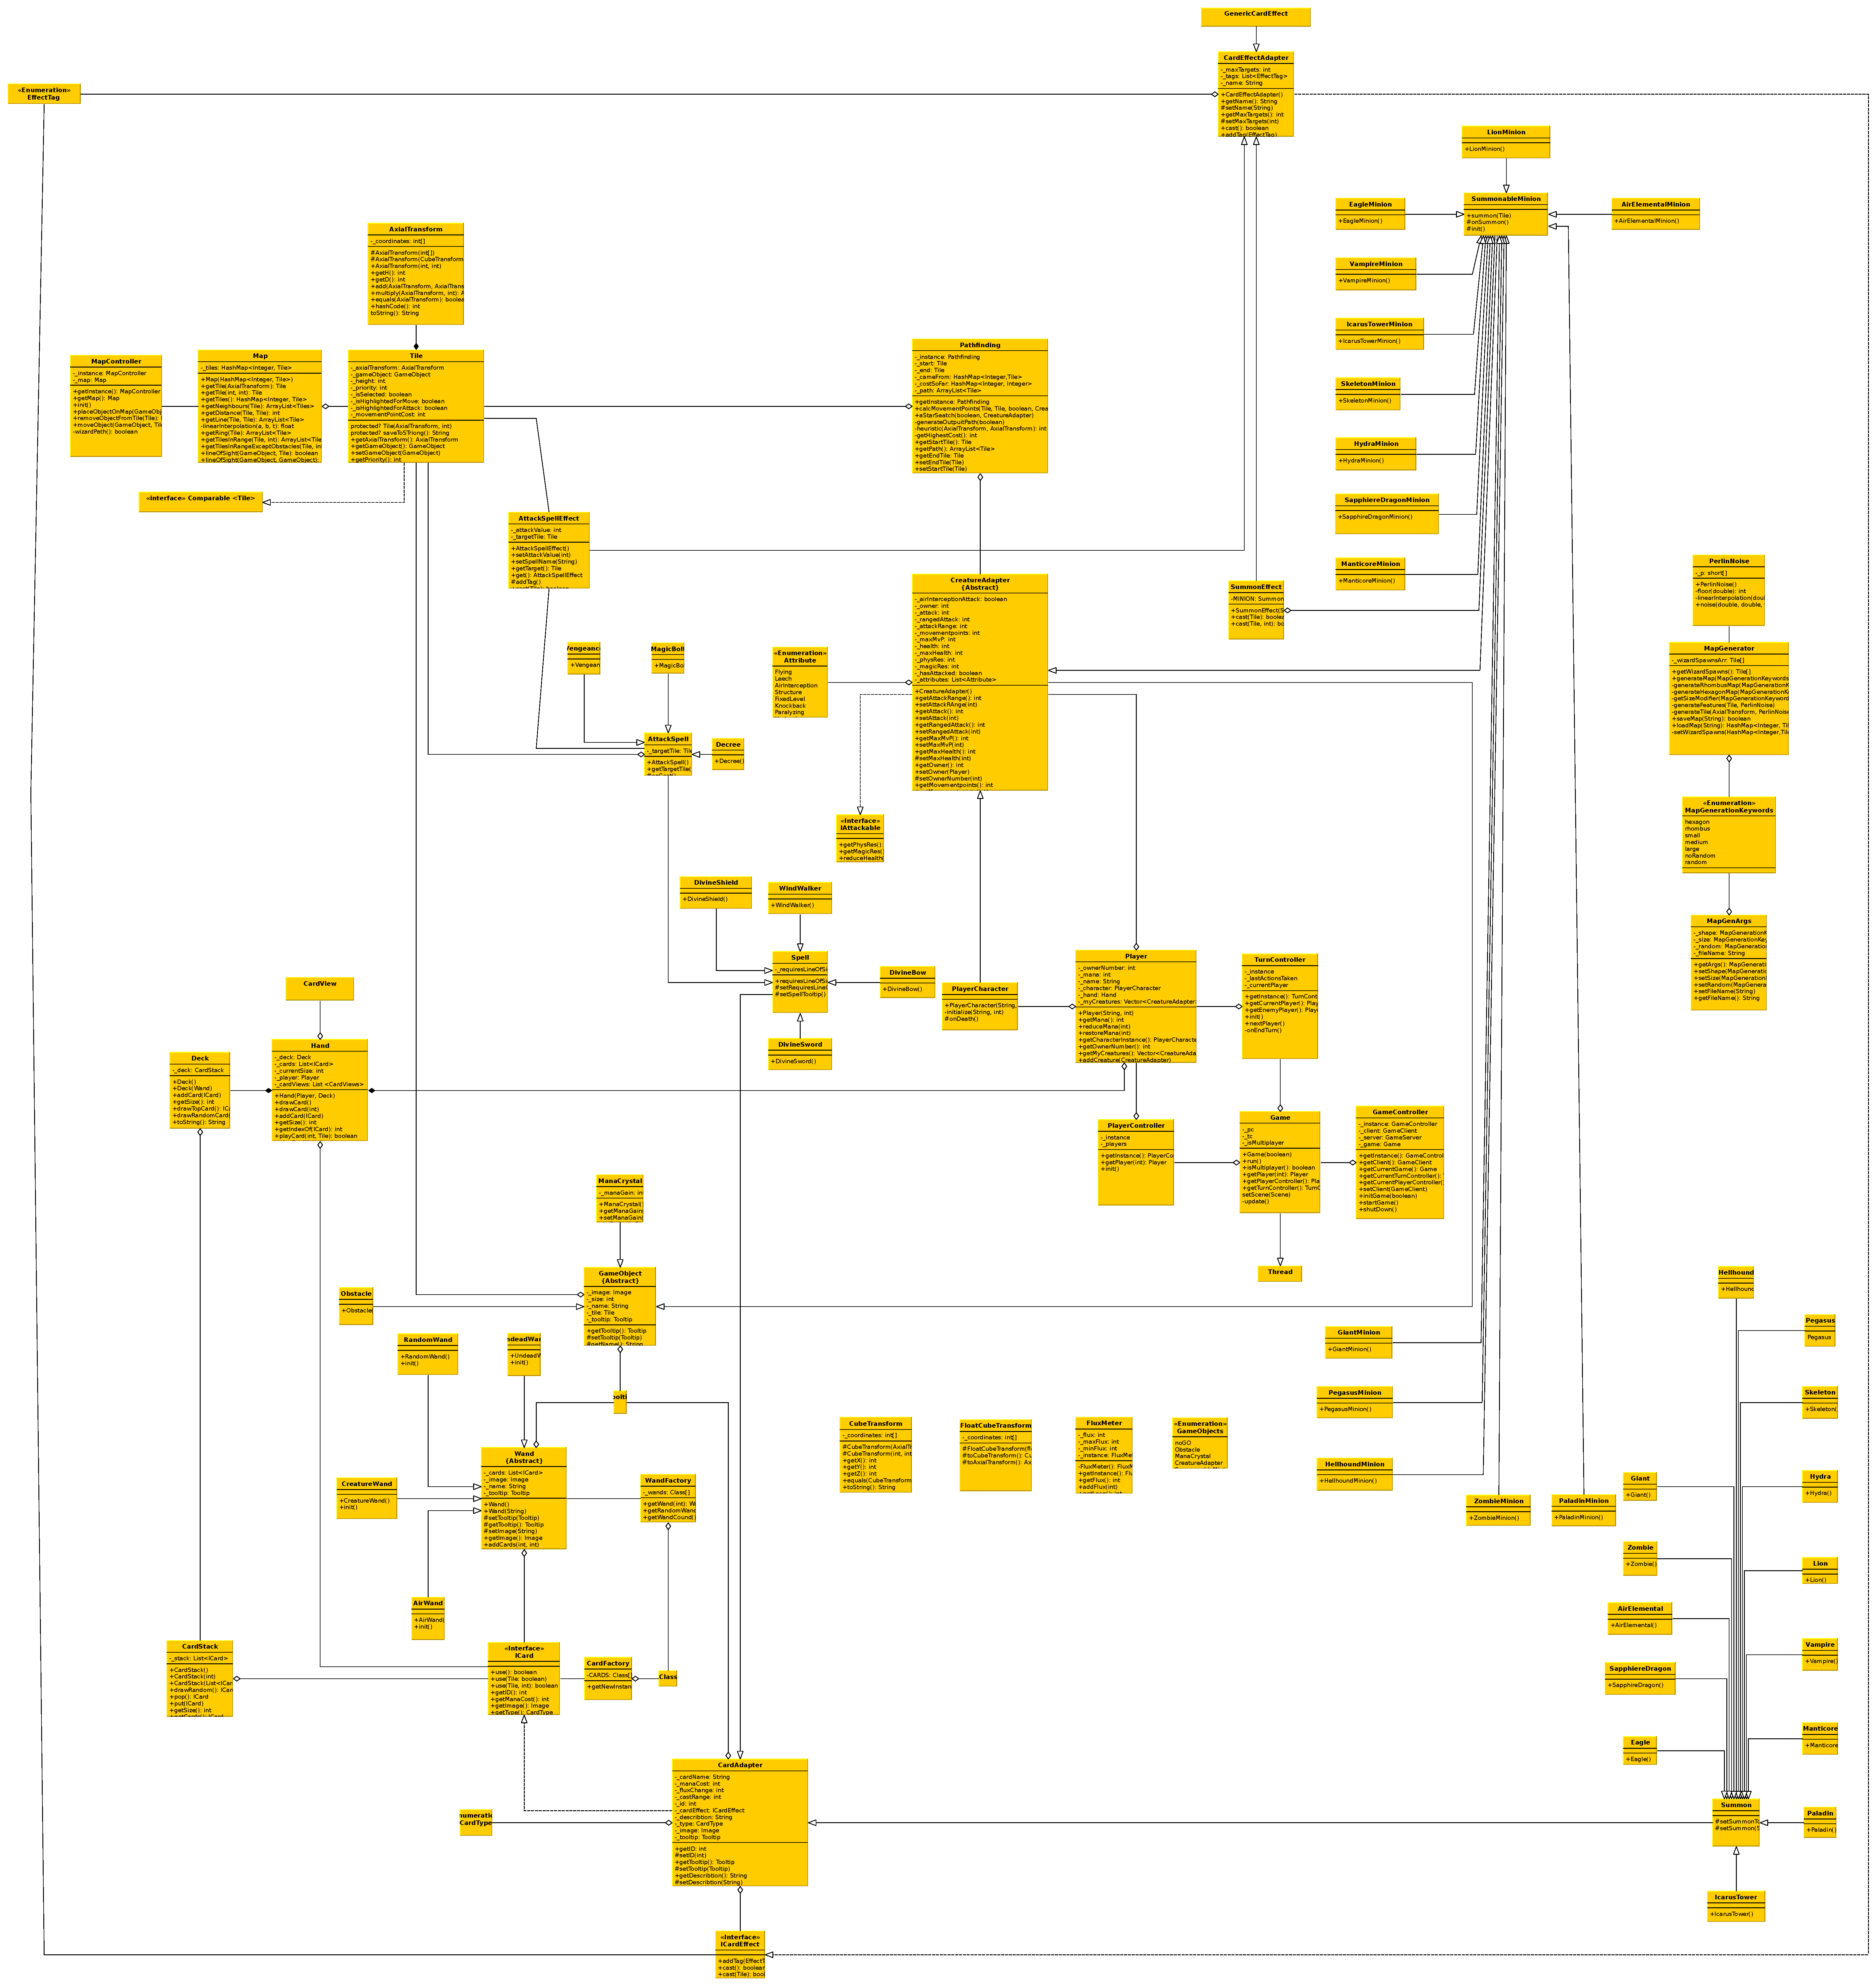
\includegraphics[width=\textwidth, height=50em]{Entwurf}
	\section{Benutzungshinweise}
	\subsection{Das Hauptmenü}
	\vspace{1em}
	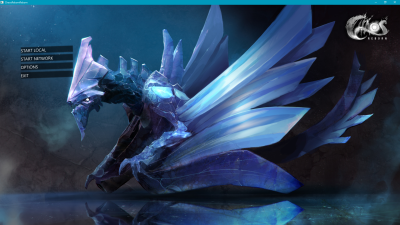
\includegraphics[width=\textwidth]{Prog2_EA_V2/screenshots/Hauptmenu1.png}\\
	
	Das Hauptmenü ist sichtbar, sobald das Spiel gestartet ist. Es stellt folgende Möglichkeiten bereit:\\
	
	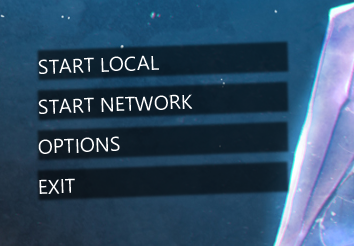
\includegraphics[width=\textwidth, height=20em]{Prog2_EA_V2/screenshots/Hauptmenu2.png}\\
	\paragraph{Ein lokales Spiel starten}
	Die Schaltfläche \glqq Start Local\grqq\hspace{0.05em}startet ein Spiel, bei dem beide Spieler an demselben Rechner gegeneinander spielen.
	Für weitere Informationen siehe Abschnitt \glqq Ein lokales Spiel starten \grqq.
	\paragraph{Ein Spiel über Netzwerk starten}
	Die Schaltfläche \glqq Start Network\grqq\hspace{0.05em} startet ein Spiel, bei dem beide Spieler über Netzwerk gegeneinander spielen.
	Für weitere Informationen siehe Abschnitt \glqq Ein Netzwerkspiel Starten\grqq\hspace{0.05em}.
	
	\paragraph{Optionen}
	Die Schaltfläche \glqq Options\grqq\hspace{0.05em} ermöglicht zugriff auf diverse Einstellungen.
	Für weitere Informationen siehe Abschnitt \glqq Die Optionen\grqq\hspace{0.05em}.
	
	\paragraph{Beenden}
	Die Schaltfläche \glqq Exit\grqq\hspace{0.05em} beendet das Spiel.
	
	\subsection{Die Optionen}
	
	\paragraph{Karteneinstellungen}
	Unter \glqq Map Options\grqq\hspace{0.05em}  kann die Karte ausgewählt werden, auf der gespielt werden soll.\\
	Für weitere Informationen siehe Abschnitt \glqq Die Karteneinstellungen\grqq\hspace{0.05em} .
	
	\paragraph{Audioeinstellungen}
	Unter \glqq Sound\grqq\hspace{0.05em}  kann die Ambientemusik aktiviert oder deaktiviert, sowie ihre Lautstärke angepasst werden.
	
	\paragraph{Zurück zum Hauptmenü}
	Ein Druck auf die \glqq Back\grqq\hspace{0.05em}  Schaltfläche bringt Sie zurück ins Hauptmenü.
	
	
	\subsubsection{Die Karteneinstellungen}
	Hier können unter drei Überschriften mittels Drop-Down-Menüs Optionen für die Karte ausgewählt werden.
	\begin{center}
		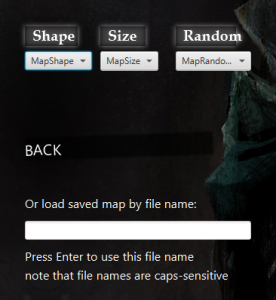
\includegraphics{Prog2_EA_V2/screenshots/Karteneinstellungen.png}
	\end{center}
	
	Werden hier keine Veränderungen vorgenommen wird eine unter \glqq Hexagonal, Medium, Not Random\grqq\hspace{0.05em}  gespeicherte Karte als Standardkarte ausgewählt.
	Sollten Veränderungen vorgenommen werden, sollten Sie dies unter allen drei Überschriften tun.
	Alternativ kann der Dateiname einer zuvor gespeicherten Karte eingegeben werden, um diese Karte zu verwenden.
	Zum Speichern von Karten finden Sie weitere Informationen unter \glqq Das Pausemenü\grqq\hspace{0.05em} .
	
	\paragraph{Kartenform}
	Unter \glqq Shape\grqq\hspace{0.05em}  Kann zwischen einer rhombusförmigen und sechseckförmigen Karte gewählt werden.
	
	\paragraph{Kartengröße}
	Unter \glqq Size\grqq\hspace{0.05em}  kann zwischen 3 unterschiedlichen Größen für Karten gewählt werden.
	
	\paragraph{Zufall}
	Unter \glqq Random\grqq\hspace{0.05em} kann zwischen \glqq Random\grqq\hspace{0.05em}  - einer zufällig generierten Karte - und \glqq Not Random\grqq\hspace{0.05em}  - einer per Hand erstellten Karte gewählt werden.
	Nicht zufällige Karten sind in allen drei Größen, jedoch nur für sechseckige Karten verfügbar.
	
	\paragraph{Namenseingabe}
	Haben Sie zuvor eine Karte abgespeichert, können sie auch im sichtbaren Textfeld deren Dateinamen (ohne Endung .map) eingeben und mittels Druck auf die Enter-Taste ihrer Tastatur bestätigen. Die entsprechende Karte wird beim Start des Spiels geladen werden.
	Sollten Sie sich umentscheiden und doch keine Karte laden wollen, entfernen Sie jeglichen Text aus dem Eingabefeld und bestätigen erneut mittels Enter.\\
	Haben Sie alle gewünschten Einstellungen vorgenommen, gelangen Sie mittels Druck auf die \glqq Back\grqq\hspace{0.05em}  Schaltfläche zurück.
	
	\subsection{Das Pausemenü}
	Das Pausemenü kann während eines Laufenden Spiels mittels Druck auf die Escape-Taste Ihrer Tastatur geöffnet werden.
	Ihnen stehen hier folgende Möglichkeiten bereit:
	
	\paragraph{Optionen}
	Ähnllich wie im Hauptmenü (siehe \glqq Das Hauptmenü\grqq) können Sie unter \glqq Optionen\grqq\hspace{0.05em} Einstellungen vornehmen.
	Beachten Sie, dass Änderungen der Karteneinstellungen während des laufenden Spieles keine Auswirkung haben.
	
	\paragraph{Eine Karte Speichern}
	Mit Auswahl der \glqq Save Map File\grqq\hspace{0.05em} Schaltfläche öffnet sich ein neues Fenster mit dem Titel \glqq Saving Map\grqq\hspace{0.05em} .
	In einem Textfeld können Sie einen Dateinamen angeben, unter dem Sie die Karte abspeichern können. 
	Ein Klick auf bestätigen schließt das Speichern ab.
	Beachten Sie, dass dies lediglich die Karte selbst, nicht den aktuellen Stand ihres Spieles sichert.
	Möchten Sie die Karte doch nicht abspeichern schließen sie dieses Fenster mit einem Klick auf das \glqq X\grqq\hspace{0.05em}  in der oberen rechten Ecke.
	
	\paragraph{Weiterspielen}
	Ein Klick auf \glqq Resume\grqq\hspace{0.05em}  setzt das laufende Spiel fort.
	
	\paragraph{Zum Hauptmenü}
	Ein Klick auf \glqq Back to Main Menu\grqq\hspace{0.05em}  bringt Sie zurück ins Hauptmenü. Dabei geht ihr aktueller Spielstand verloren.
	
	\begin{center}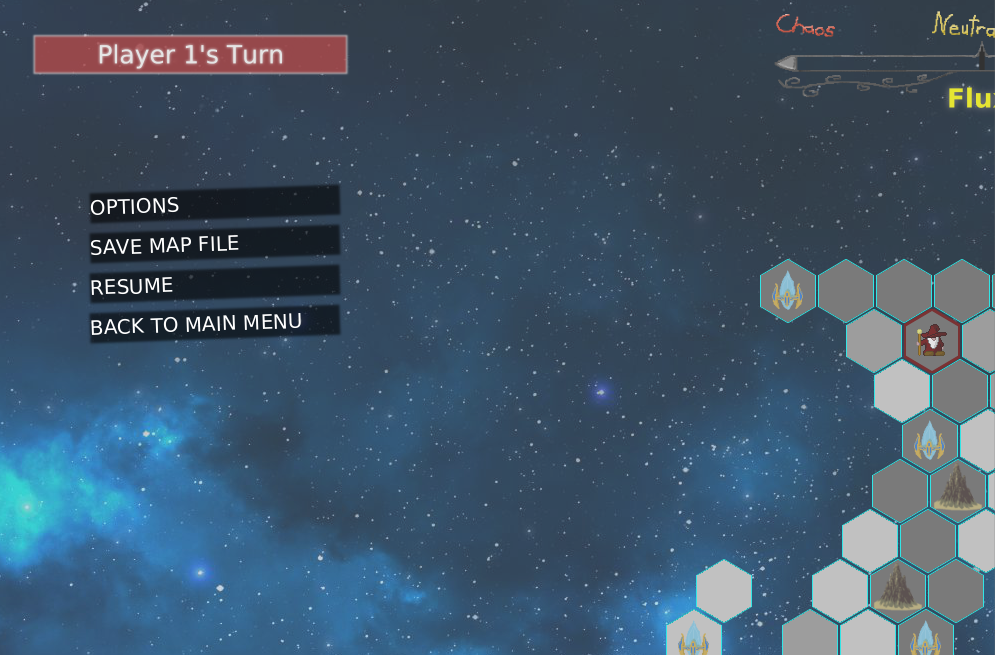
\includegraphics[width=\textwidth]{Prog2_EA_V2/screenshots/Pausemenu.png}\end{center}
	
	\subsection{Ein lokales Spiel starten}
	Im lokalen Spiel spielen beide Kontrahenten an einem Rechner und wechseln zwischen Ihren Zügen die Kontrolle über Maus und Tastatur ab.
	Nachdem Sie im Hauptmenü auf die Schaltfläche \glqq Start Local\grqq\hspace{0.05em}  geklickt haben, gelangen Sie zunächst in ein Auswahlmenü für den Zauberstab beider Spieler.
	
	\begin{center}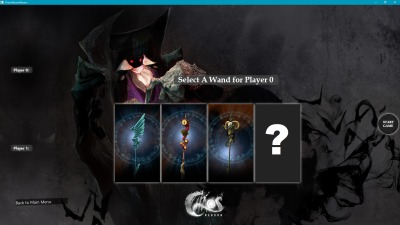
\includegraphics[width=\textwidth]{Prog2_EA_V2/screenshots/LokalesSpiel1.png}
	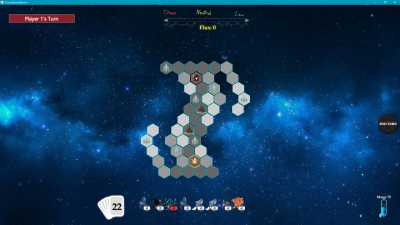
\includegraphics[width=\textwidth]{Prog2_EA_V2/screenshots/Spiel1.png}\end{center}
	Beide Spieler wählen hier den Zauberstab aus, mit dem Sie das Spiel bestreiten möchten. In der oberen rechten Ecke des Bildschirmes wird dabei angezeigt welche Spielkarten wie oft im Deck eines Stabes enthalten sind.
	Die \glqq Random Wand\grqq\hspace{0.05em} auszuwählen weist dem Spieler erst zu Spielbeginn einen zufälligen Zauberstab zu.
	Mehr Informationen zu Zauberstäben und Spielkarten finden Sie unter \glqq Die Spielmechanik\grqq\hspace{0.05em}.
	Sobald beide Spieler mit ihrer Wahl zufrieden sind klicken Sie auf \glqq Start Game\grqq\hspace{0.05em}.
	Wie gespielt wird erfahren Sie unter \glqq Das Spiel\grqq\hspace{0.05em}.
	Zu jedem Zeitpunkt der Vorbereitung gelangen Sie durch einen Klick auf \glqq Back to Main Menu\grqq\hspace{0.05em} zurück ins Hauptmenü.
	
	\subsection{Ein Netzwerkspiel starten}
	Möglicherweise sind für das Spiel über Netzwerk Portfreigaben in ihrem Router und/oder ihrer Firewall nötig. Das Spiel verwendet den Port 6066.\\
	Um ein Netzwerkspiel zu starten, öffnen Sie zunächst das Spiel auf zwei Rechnern oder starten das Spiel auf demselben Rechner zweimal.\\
	Zunächst klicken Sie in einem Spiel auf \glqq Host\grqq\hspace{0.05em}.
	Ihnen werden nun Verbindungsinformationen angezeigt, mittels derer ein zweiter Spieler Ihrem Spiel beitreten kann.
	Im anderen Spiel klicken sie auf die Schaltfläche \glqq Join\grqq\hspace{0.05em}, um einem Spiel beizutreten.
	Es erscheint ein Textfeld zur Eingabe der IP-Adresse des Hosts.
	Sind beide Spiele auf demselben Rechner gestartet geben Sie hier \glqq localhost\grqq\hspace{0.05em} ein.
	Andernfalls geben Sie die IP-Adresse des Hosts ein.
	Bestätigen Sie die Eingabe mittels Druck auf die Enter-Taste oder \glqq Join Game!\grqq\hspace{0.05em} Schaltfläche.
	Wurde die Verbindung erfolgreich hergestellt, gelangen beide Spieler in ein Auswahlmenü für Ihren Zauberstab.
	Hat ein Spieler seine Auswahl getroffen klickt er auf \glqq Ready\grqq\hspace{0.05em}.
	Haben beide Spieler dies getan, beginnt das Spiel.
	Wie gespielt wird erfahren Sie unter \glqq Das Spiel\grqq\hspace{0.05em}.
	Falls sie eine eigens erstellte Map bespielen wollen muss diese von beiden Spielern geladen werden.
	
	\subsection{Das Spiel}
	
	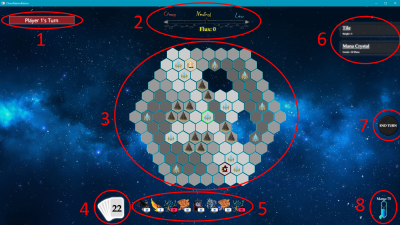
\includegraphics[width=\textwidth]{Prog2_EA_V2/screenshots/DsaSpiel2.png}
	
	\paragraph{(1) Zugspieler-Anzeige}
	Hier sehen Sie, welcher Spieler derzeit am Zug ist.
	
	\paragraph{(2) Mana-Flux-Anzeige}
	Hier sehen Sie, den aktuellen Stand des Flux; ob es gerade in Richtung Chaos oder Rechtschaffenheit verschoben oder neutral ist.
	
	\paragraph{(3) Das Spielfeld}
	Das Spielfeld zeigt ihnen die Karte, auf der Sie spielen, sowie die Positionen von Zauberern, Kreaturen, Hindernissen und Manakristallen.
	Sie können einzelne Felder (Sechsecke) mit der linken Maustaste anklicken, um sie Auszuwählen. Dies hebt dieses Feld grün hervor.
	Sie können die Position des Spielfeldes auf dem Bildschirm verändern indem sie es per drag-and-drop über den Bildschirm ziehen.
	
	\paragraph{(4) Das Deck}
	Hier können Sie sehen, wie viele Karten noch in Ihrem deck vorhanden sind.
	
	\paragraph{(5) Die Hand}
	Die Hand zeigt Ihnen, welche Karten sie gezogen haben, wie viel Mana diese kosten (blaue Zahl) und ob sie diese gerade ausspielen können (haben Sie zu wenig Mana werden die Kosten einer Karte rot markiert).
	Außerdem wird ihnen, falls das Flux nicht neutral ist, die Kosten welcher Karten derzeit durch das Flux beeinflusst werden.
	
	\paragraph{(6) Tooltips}
	In der rechten, oberen Ecke werden Ihnen Tips zu dem Feld oder Zauber angezeigt, das oder den Sie derzeit ausgewählt haben.
	Befindet sich auf dem ausgewählten Feld eine Kreatur, werden auch zu ihr hier Informationen angezeigt.
	
	\paragraph{(7) Zug-Beenden-Schaltfläche}
	Ein klick auf \glqq End Turn\grqq\hspace{0.05em} beendet Ihren Zug. Nun ist ihr Kontrahent an der Reihe.
	
	\paragraph{(8) Mana-Anzeige}
	Hier sehen Sie, wie viel Mana Sie derzeit zur Verfügung haben, um Zauber auszuspielen oder Kreaturen zu beschwören.
	
	\subsubsection{Eine Bewegung ausführen}
	Um eine Kreatur, oder Ihren Zauberer zu bewegen, wählen Sie zunächst mit der linken Maustaste das Feld auf dem sich die Kreatur befindet aus.
	Daraufhin werden ihnen in hellgrün alle Felder hervorgehoben, zu denen sich diese Kreatur bewegen kann.
	Mit einem Rechtsklick auf eines dieser Felder bewegen Sie die Kreatur dorthin.
	
	\subsubsection{Einen Manakristall einsammeln}
	Um einen Kristall einzusammeln, bewegen Sie eine Ihrer Kreaturen auf das Feld, auf dem sich der Kristall befindet.
	Der Kristall verschwindet und Ihnen wird Mana gutgeschrieben.
	Eine Bewegung, die lediglich über einen Kristall hinweg verläuft sammelt diesen nicht ein.
	
	\subsubsection{Einen Angriff ausführen}
	Um eine feindliche Kreatur anzugreifen wählen Sie zunächst wieder mit Linksklick ein Feld, auf dem sich eine Ihrer eigenen Kreaturen befindet.
	Nun bewegen Sie Ihre Kreatur auf ein Feld, von dem aus es den Feind angreifen kann. 
	Wählen Sie erneut das Feld, ihrer eigenen Kreatur aus. Jetzt wird ihnen das Feld, auf dem sich der Feind befindet rot hervorgehoben. 
	Rechtsklicken Sie auf dieses um den Angriff auszuführen.
	Alternativ können Sie auch, wenn bereits Felder mit Gegnerischen Kreaturen hervorgehoben werden, nachdem Sie zum ersten Mal Ihre Kreatur wählen, sofort auf den Gegner Rechtsklicken. Ihre Kreatur wird sich nun so weit bewegen wie nötig, um den Angriff durchzuführen. 
	\subsubsection{Eine Spielkarte verwenden}
	Linksklicken sie zunächst auf auf die Karte in Ihrer Hand.
	Es werden ihnen mögliche Zielfelder in rot hervorgehoben.
	Linksklicken Sie eines dieser Felder, um die Karte auszuspielen.
	
	\subsection{Die Spielmechanik}
	\subsubsection{Spielziel}
	Ziel des Spieles ist es den feindlichen Zauberer zu besiegen, indem seine Lebenspunkte auf 0 reduziert werden.
	
	\subsubsection{Zauberstäbe}
	
	\subsubsection{Die Hand \& Das Deck}
	Der Zauberstab bestimmt, welche Spielkarten wie oft im Deck des Spielers vorkommen. Das Deck enthält diese Karten in zufälliger Reihenfolge.
	Die Hand besteht aus Karten, die vom Deck gezogen werden. Zu Beginn jedes Zuges wird eine neue Karte gezogen.
	Ist das Deck leer, bleiben nur noch die Karten in der Hand. Ist auch diese leer bleibt nur zu hoffen, dass die Kreaturen auf dem Feld zum Sieg reichen...
	
	\subsubsection{Der eigene Zauberer}
	Der Zauberer selbst hat dieselben Werte und Attribute wie andere Kreaturen auch (siehe Abschnitt \glqq Kreaturen\grqq\hspace{0.05em}). Sinken die Lebenspunkte des Zauberers auf oder unter 0 ist das Spiel verloren.
	
	\subsubsection{Angirffe \& Bewegungen}
	\paragraph{Bewegung}
	Kreaturen können sich abhängig von ihren Bewegungspunkten unterschiedlich weit über die Karte bewegen. 
	Bewegungen werden durch die Gegebenheiten der Karte eingeschränkt. So können sich Kreaturen nicht über Hindernisse hinweg bzw. durch sie hindurch bewegen.\\
	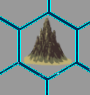
\includegraphics[width=\textwidth]{Prog2_EA_V2/screenshots/Hindernis.png}
	
	Außerdem haben Felder der Karte unterschiedliche Höhen. Ist der unterschied zweier aneinander grenzender Felder größer als 1, kann die Höhendifferenz von einer Kreatur nicht überwunden werden (es gibt Ausnahmen, siehe \glqq Attribute\grqq\hspace{0.05em}).\\
	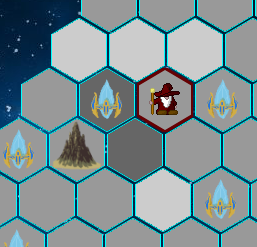
\includegraphics[width=\textwidth]{Prog2_EA_V2/screenshots/Hoehen.png}
	
	Sich auf einen Manakristall zu bewegen sammelt diesen für den Spieler ein (siehe \glqq Mana \& Flux\grqq\hspace{0.05em}).
	
	
\includegraphics[width=\textwidth]{Prog2_EA_V2/screenshots/Manakristall.png}
	
	\paragraph{Angriff}
	Es wird unterschieden zwischen Nah- und Fernkampfangriffen. 
	Ein Nahkampfangriff kann gegen eine angrenzende Kreatur ausgeführt werden.
	Nahkampfangriffe fügen sowohl dem Angreifer, als auch dem Verteidiger schaden zu.
	Bei Fernkampfangriffen erleidet nur der Verteidiger Schaden.
	Um einen Fernkampfangriff auszuführen, muss der Angreifer das Ziel sehen können. Das bedeutet, dass sich zwischen ihm und dem Ziel keine Hindernisse befinden und dass zwischen ihnen keine Felder höher gelegen sind als beide Kreaturen groß sind.
	
	\subsubsection{Zauberei}
	\paragraph{Kreaturen beschwören}
	beschworene Kreaturen sind austauschbare Kämpfer, deren Verlust nicht zum Verlieren des Spiels führt. Sie können sich bewegen, angreifen und angegriffen werden.
	
	\subsubsection{Zaupersprüche}
	Zaubersprüche unterstützen den Spieler, indem Sie eine Kreatur verletzen, den eigenen Zauberer stärken oder den Gegner Karten abwerfen lassen.
	Magischer Schlag (\glqq Magic Bolt\grqq\hspace{0.05em})
	Der Magische Schlag verursacht Schaden an der Zielkreatur. 
	
	\paragraph{Rache (\glqq Vengeance \grqq\hspace{0.05em})}
	Rache verursacht Schaden an der Zielkreatur. Handelt es sich dabei um den gegnerischen Zauberer wirft der Gegner stattdessen 2 Karten aus seiner Hand ab.
	
	\paragraph{Erlass (\glqq Decree\grqq\hspace{0.05em})}
	Erlass verursacht Schaden an der Zielkreatur. Handelt es sich dabei um den gegnerischen Zauberer wirft der Gegner stattdessen 2 Karten aus seiner Hand ab.
	
	\paragraph{Windläufer (\glqq Windwalker\grqq\hspace{0.05em})}
	Windläufer erhöht die maximalen Bewegungspunkte des Zauberers um 1 und verleiht ihm das Attribut Fliegend. Wird der Zauber ein zweites Mal gespielt erhält der Zauberer den Bewegungspunkt, jedoch keine weiteren Attribute.
	
	\paragraph{Göttlicher Schild (\glqq Divine Shield\grqq\hspace{0.05em})}
	Göttlicher Schild erhöht die Physische Verteidigung des Zauberers.
	
	\paragraph{Göttlicher Bogen (\glqq Divine Bow\grqq\hspace{0.05em})}
	Göttlicher Bogen verleiht dem Zauberer einen Fernkampfangriff mit einer Reichweite von 3 Wird der Zauber ein zweites Mal gespielt steigt der Fernkampfangriffswert, jedoch nicht die Reichweite.
	
	\paragraph{Göttliches Schwert (\glqq Divine Sword\grqq\hspace{0.05em})}
	Göttliches Schwert erhöht den Angriffswert des Zauberers.
	
	\subsubsection{Kreaturen}
	\paragraph{Werte}:\newline
	\paragraph{Lebenspunkte (\glqq Health\grqq\hspace{0.05em})}
	Lebenspunkte geben an, wie verletzt eine Kreatur ist. Sinken sie auf oder unter 0, ist die Kreatur besiegt und wird vom Spielfeld entfernt.
	
	\paragraph{Größe (\glqq Size\grqq\hspace{0.05em})}
	Die Größe einer Kreatur wird verwendet um zu bestimmen, ob sie im Fernkampf angegriffen werden oder angreifen kann; genauer: ob sie als Ziel gesehen werden oder ihr Ziel sehen kann.
	
	\paragraph{Angriff (\glqq Attack\grqq\hspace{0.05em})}
	Der Anriffswert einer Kreatur bestimmt, wie viel Schaden sie im Nahkampf verursacht, h.h. wie viele Lebenspunkte der Gegner verliert, wenn sie kämpft.
	
	\paragraph{Angriffsreichweite (\glqq Attack Range\grqq\hspace{0.05em})}
	Die Angriffsreichweite gibt an, wie weit das Ziel eines Angriffes von der Kreatur entfernt sein kann. Eine 1 bedeutet, dass die Kreatur nur Feinde auf angrenzenden Feldern angreifen kann.
	
	\paragraph{Fernkampfangriff (\glqq Ranged Attack\grqq\hspace{0.05em})}
	Hat eine Kreatur eine Angriffsreichweite größer als 1, kann sie einen Fernkampfangriff durchführen. Hierbei wird zur Berechnung des Schadens der Fernkampfangriff, statt des Angriffs verwendet.
	
	\paragraph{Physische Verteidigung (\glqq Physical Resistance\grqq\hspace{0.05em})}
	Die Physische Verteidigung verringert den Schaden, den eine Kreatur durch einen Nah- oder Fernkampfangriff erleidet.
	
	\paragraph{Magische Verteidigung (\glqq Magical Resistance\grqq\hspace{0.05em})}
	Die Magische Verteidigung verringert den Schaden, den eine Kreatur durch Zaubersprüche erleidet.
	
	\paragraph{Bewegungspunkte (\glqq Movement Points\grqq\hspace{0.05em})}
	Die Bewegungspunkte geben an, wie weit eine Kreatur sich bewegen kann. Von einem Feld auf ein angrenzendes zu wechseln kostet einen Punkt, weitere Bewegungen entsprechend mehrere Punkte.
	
	\subsubsection{Attribute}
	
	\paragraph{Fliegend (\glqq Flying\grqq\hspace{0.05em})}
	Fliegende Kreaturen können bei Bewegungen Höhenunterschiede größer als 1 überwinden.\\
	\begin{center}
		
\includegraphics{Prog2_EA_V2/Art/Pegasus.png}\end{center}
	
	\paragraph{Blutsauger (\glqq Leech\grqq\hspace{0.05em})}
	Kreaturen mit Blutsauger heilen bei einem Nahkampfangriff schaden, den sie dem Ziel zufügen.\\
	\begin{center}
\includegraphics{Prog2_EA_V2/Art/Vampire.png}\end{center}
	
	\paragraph{Luftabfangen (\glqq Air Interception\grqq\hspace{0.05em})}
	Kreaturen mit diesem Attribut können einmal pro gegnerischem Zug einen zusätzlichen Angriff gegen eine Fliegende Kreatur ausführen, die eine Bewegung innerhalb ihrer Reichweite beginnt.
	
	\paragraph{Struktur (\glqq Structure\grqq\hspace{0.05em})}
	Strukturen sind gegen Zaubersprüche immun.
	
	\paragraph{Feste Höhe (\glqq Fixed Level\grqq\hspace{0.05em})}
	Die Kreatur kann keine Höhenunterschiede überwinden.\\
	\begin{center}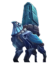
\includegraphics{Prog2_EA_V2/Art/IcarusTower.png}\end{center}
	
	\paragraph{Rückstoß (\glqq Knockback\grqq\hspace{0.05em})}
	Die Kreatur \glqq schubst" das Ziel eines Angriffes um ein Feld zurück, falls dieses frei ist und das Ziel den Angriff überlebt.\\
	\begin{center}
\includegraphics{Prog2_EA_V2/Art/AirElemental.png}\end{center}
	
	\paragraph{Paralysierend (\glqq Paralyzing\grqq\hspace{0.05em})}
	Führt eine Kreatur mit Paralysierend einen Fernkampfangriff aus, erhält das Ziel für eine Runde das Attribut Paralysiert.\\
	\begin{center}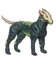
\includegraphics{Prog2_EA_V2/Art/Hellhound.png}\end{center}
	
	\paragraph{Paralysiert (\glqq Paralyzed\grqq\hspace{0.05em})}
	Eine Paralysierte Kreatur kann sich nicht bewegen und keine Angriffe ausführen.
	
	\paragraph{Untot (\glqq Undead\grqq\hspace{0.05em})}
	Eine Untote Kreatur kann nur durch andere Untote Kreaturen oder solche mit dem Attribut Untotschlächter verletzt werden.\\
	\begin{center}
\includegraphics{Prog2_EA_V2/Art/Zombie.png}\end{center}
	
	\paragraph{Untotschlächter (\glqq Undead Slayer\grqq\hspace{0.05em})}
	Die Kreatur ist selber nicht Untot, kann jedoch Untote Kreaturen verletzen.\\
	\begin{center}
\includegraphics{Prog2_EA_V2/Art/Paladin.png}\end{center}
	
	\paragraph{Einzelschuss (\glqq One Time Shot\grqq\hspace{0.05em})}
	Die Kreatur kann, solange sie auf dem Spielfeld ist, einen einzigen Fernkampfangriff ausführen, statt beliebig viele.\\
	\begin{center}
\includegraphics{Prog2_EA_V2/Art/Giant.png}\end{center}
	
	\subsubsection{Mana \& Flux}
	\paragraph{Mana}
	Kreaturen zu beschwören oder Zaubersprüche auszuspielen benötigt Mana. Die kosten hängen von der Jeweiligen Spielkarte und dem Aktuellen Flux (siehe \glqq Flux\grqq\hspace{0.05em}) ab.
	Jeder Spieler erhält zu Beginn seines Zuges Mana. Außerdem kann Mana durch das einsammeln von Manakristallen erhalten werden.\\
	\begin{center}
\includegraphics{Prog2_EA_V2/Art/Mana_Crystal.png}\end{center}
	\paragraph{Flux}
	Jede Spielkarte ist entweder rechtschaffen, neutral oder chaotisch.
	Eine rechtschaffene oder chaotische Karte auszuspielen verschiebt das aktuelle Flux in die entsprechende Richtung.
	Ist das Flux chaotisch, sind chaotische Karten für geringere Manakosten einsetzbar. Ist das Flux rechtschaffen, sind diese Karten günstiger.
	Neutrale Karten kosten immer gleich viel Mana und haben keinen Einfluss auf das Flux.\\
	\begin{center}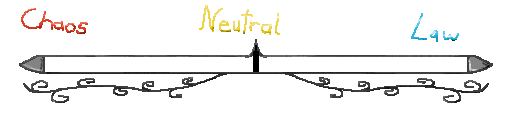
\includegraphics{Prog2_EA_V2/Art/Flux.png}\end{center}
	
	\newpage
	\section{Anwendungsbeispiel}
	Nach dem man, wie in den Benutzungshinweisen beschrieben, ein lokales Spiel gestartet und die Zauberstäbe ausgewählt hat landet man im Spiel.\\
\begin{center}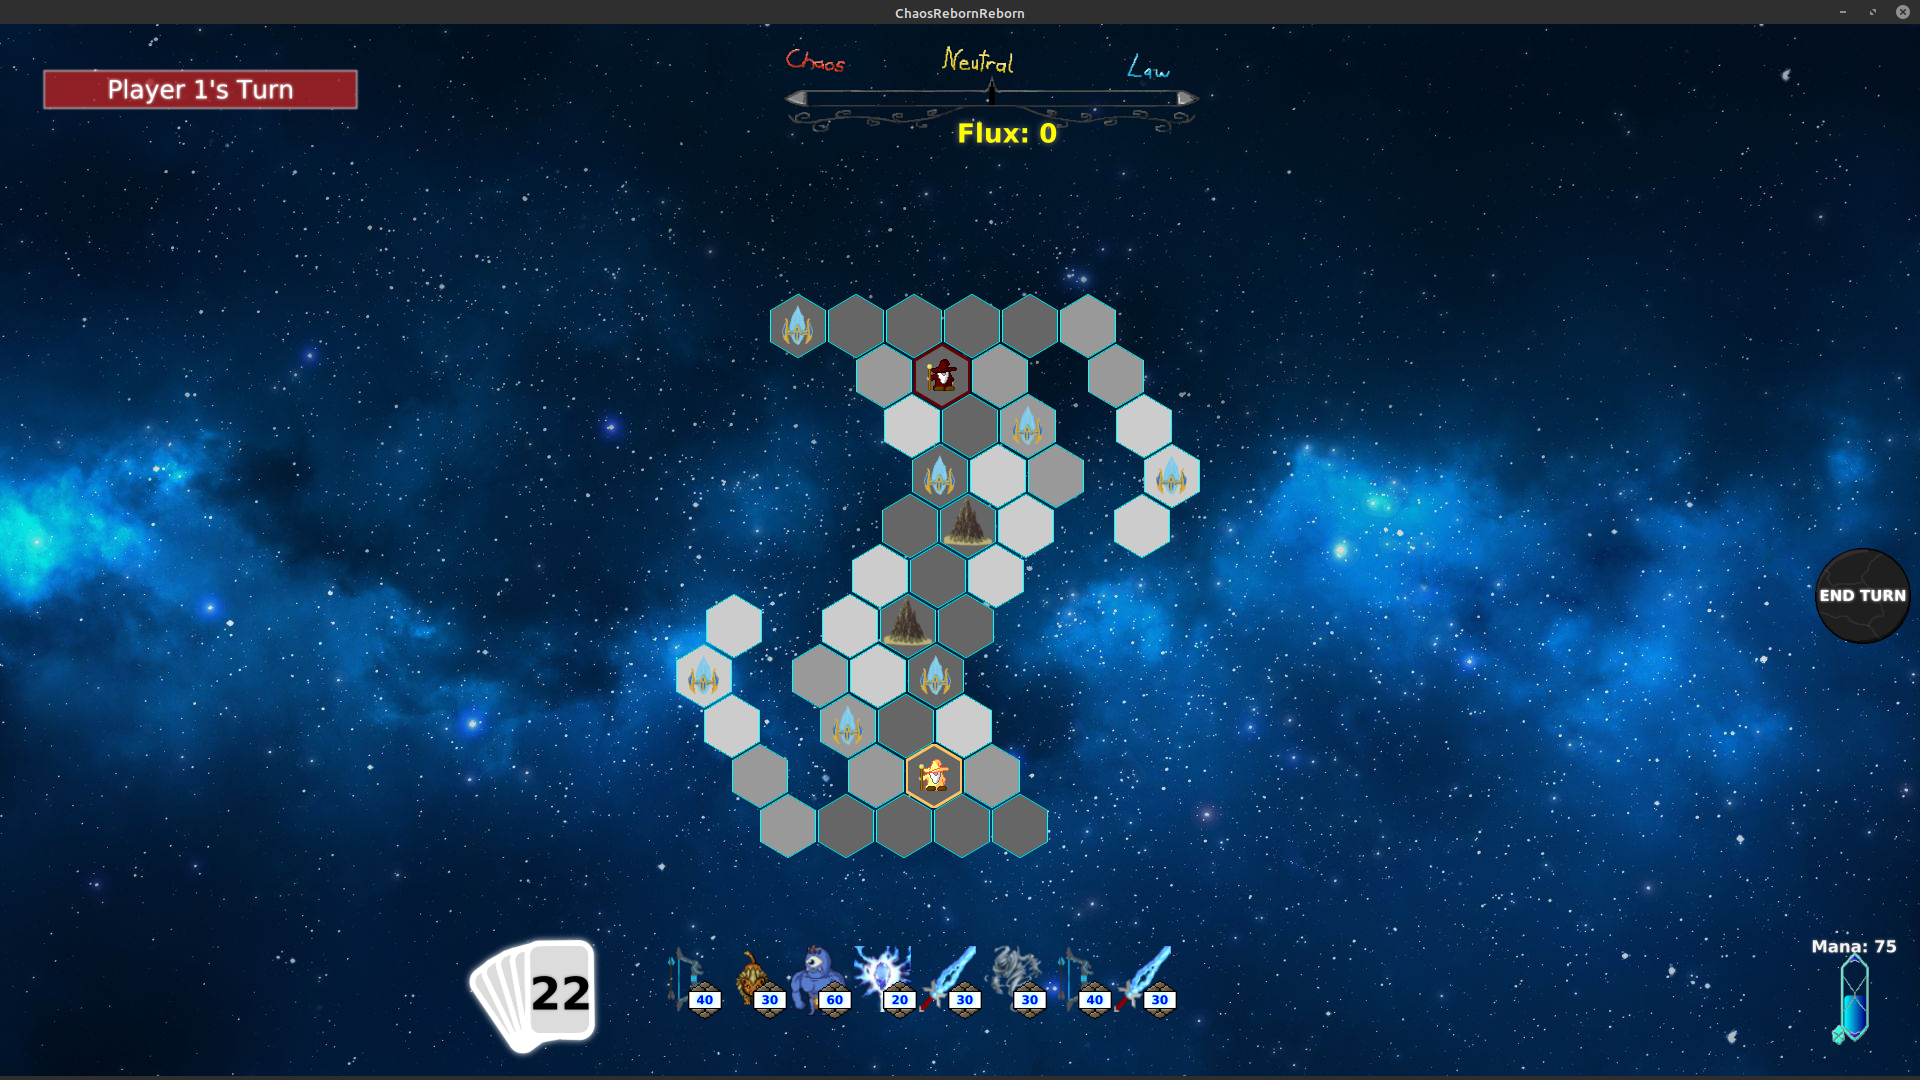
\includegraphics[width=\textwidth]{Prog2_EA_V2/screenshots/Anwendung1.png}\end{center}
	Es ist Spieler 1 am Zug, das ist der rot gekleidete Zauberer. Der Zauberer wird bewegt, zum Beispiel auf eines der Felder mit Mana das er dann einsammelt.\\
	\begin{center}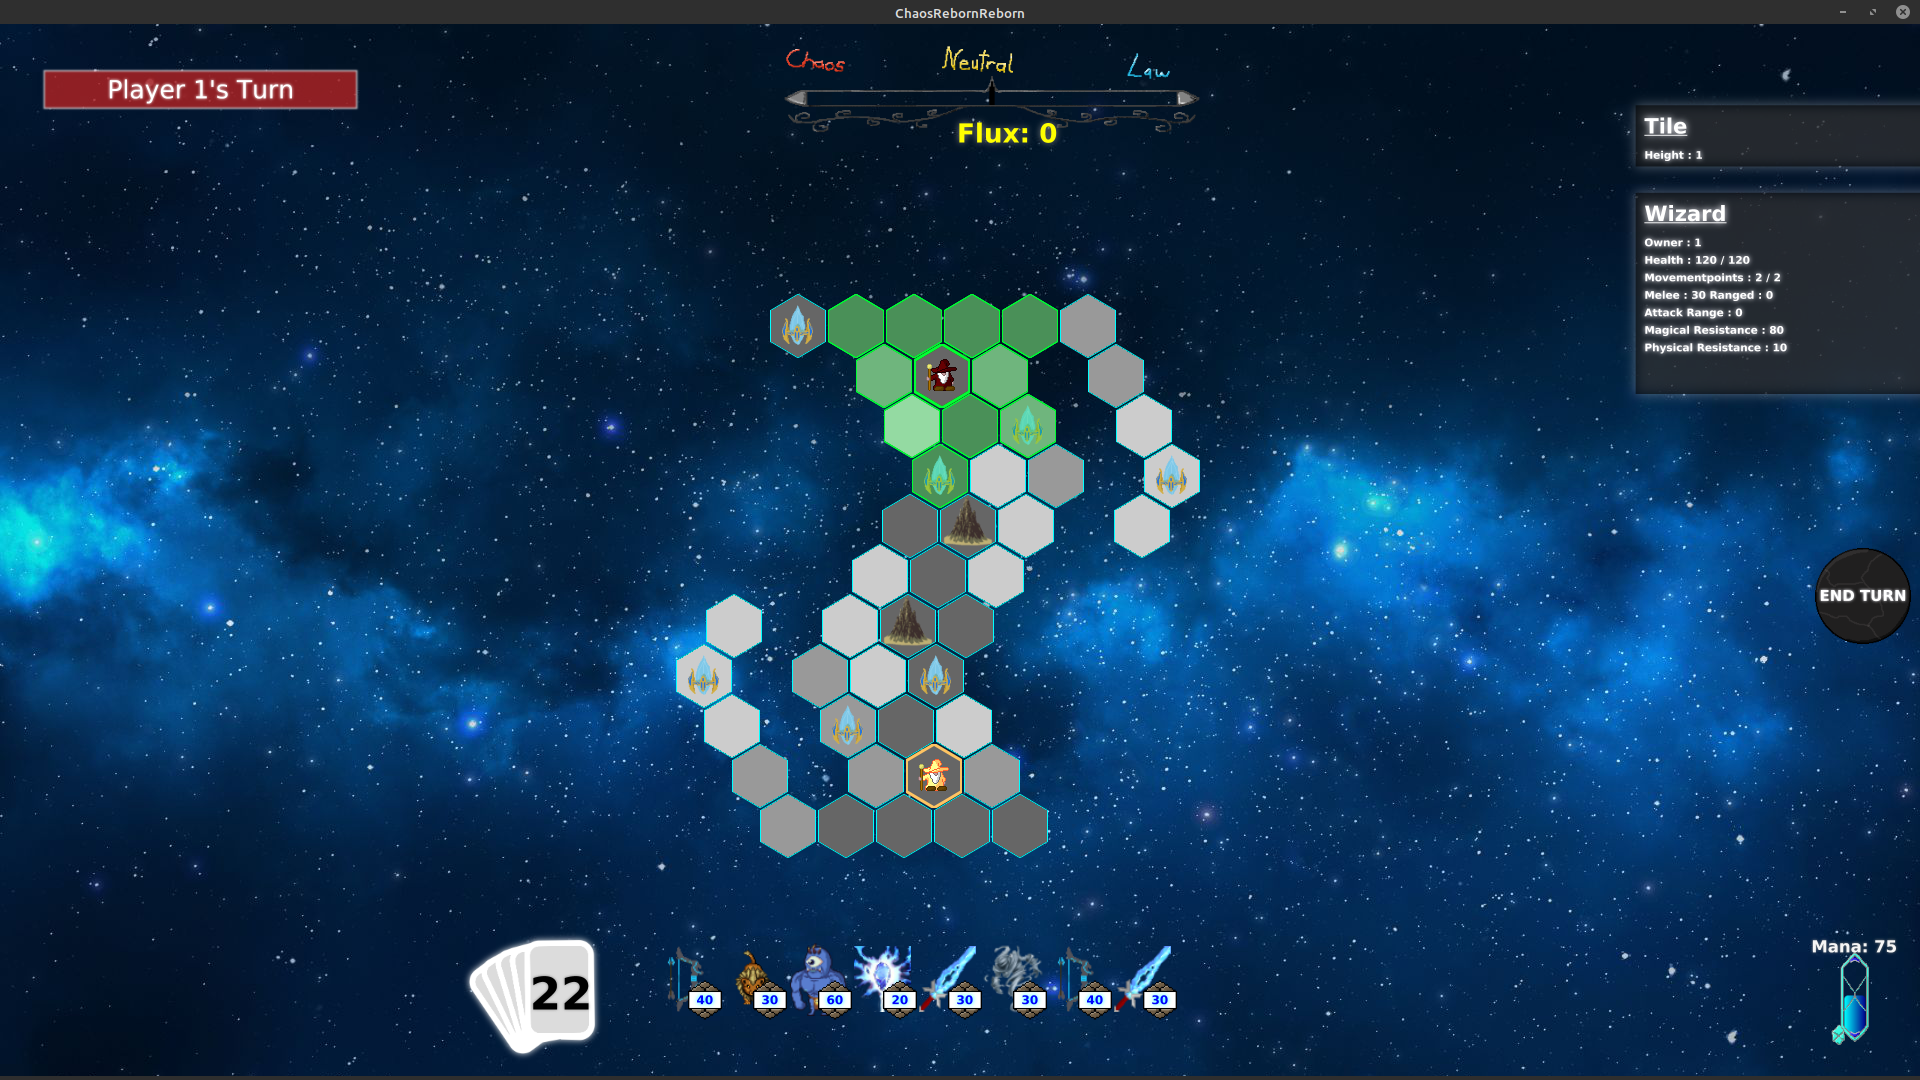
\includegraphics[width=\textwidth]{Prog2_EA_V2/screenshots/Anwendung2.png}\end{center}
	\begin{center}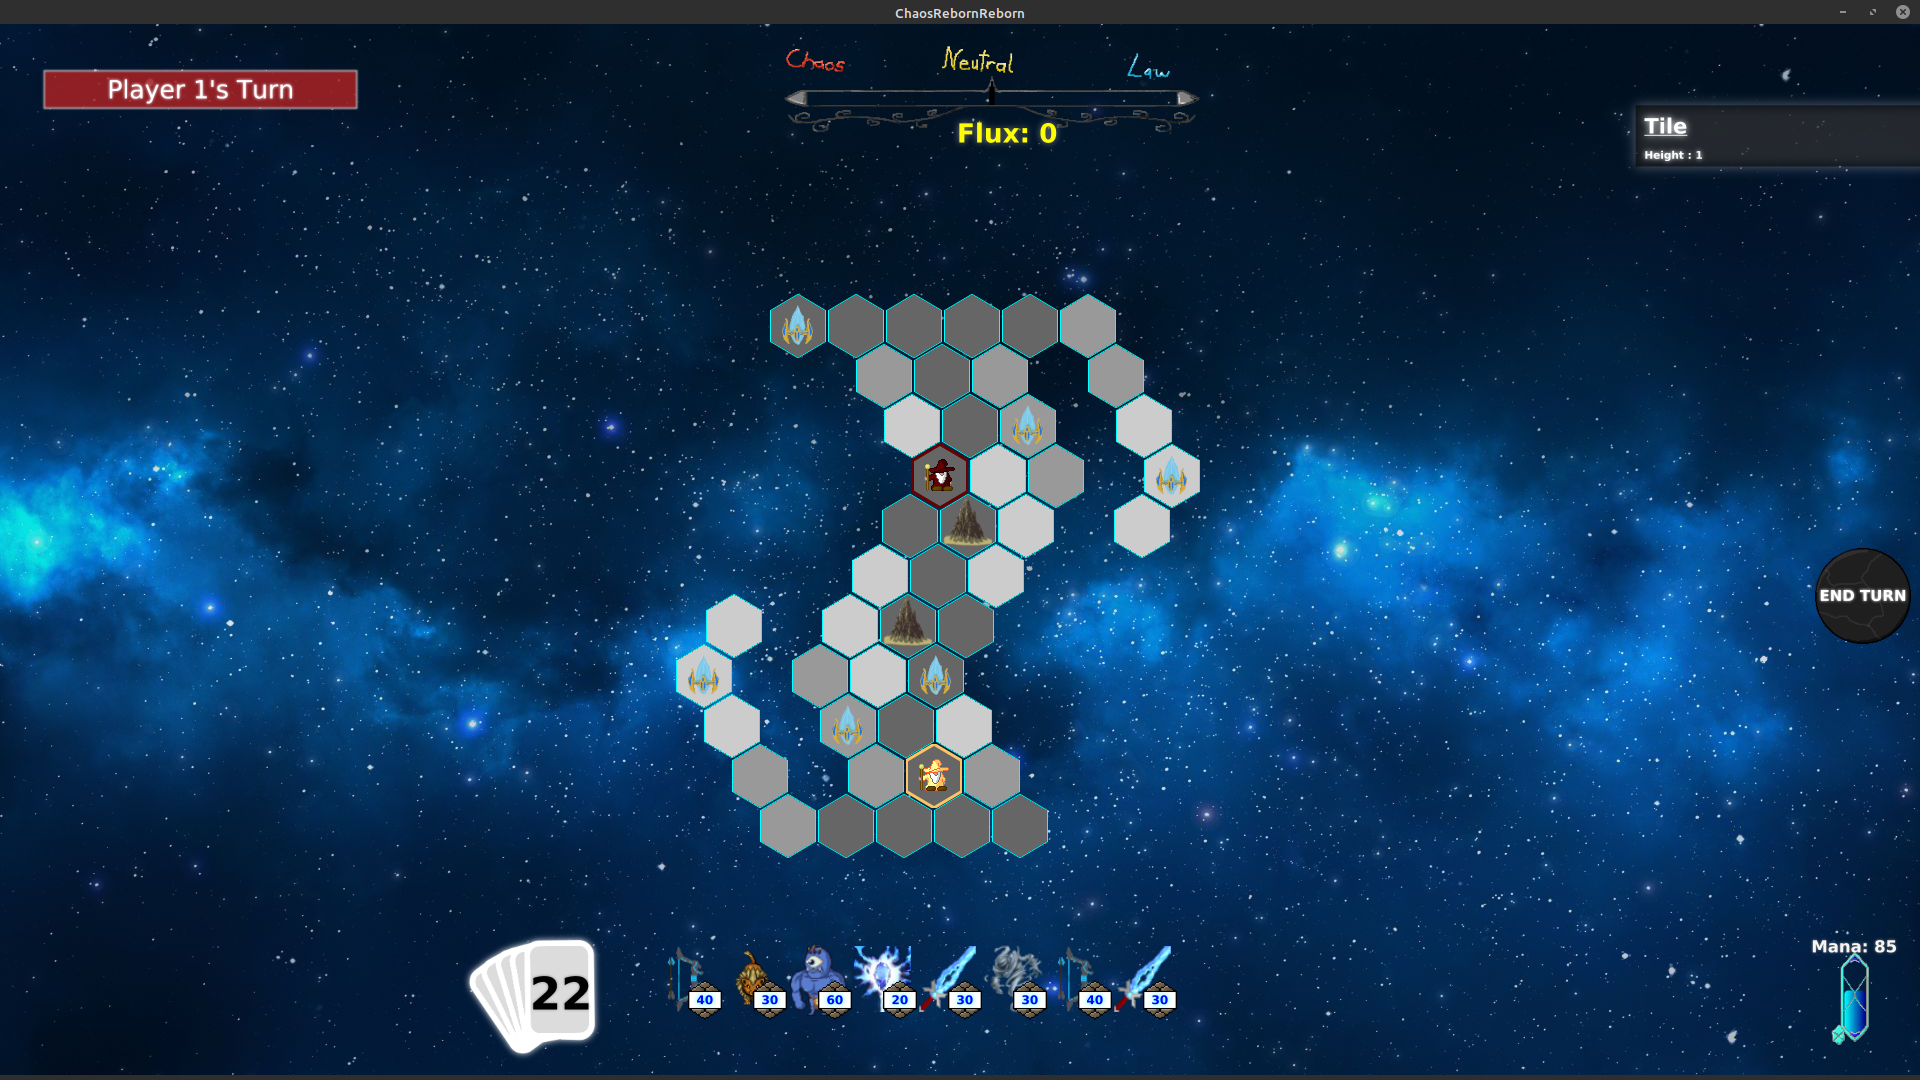
\includegraphics[width=\textwidth]{Prog2_EA_V2/screenshots/Anwendung3.png}\end{center}
	Weil kein Gegner in der Nähe ist kann der Zauberer nicht angreifen, er spielt ein paar Karten aus und platziert damit eigene Kreaturen um sich herum um.
	\begin{center}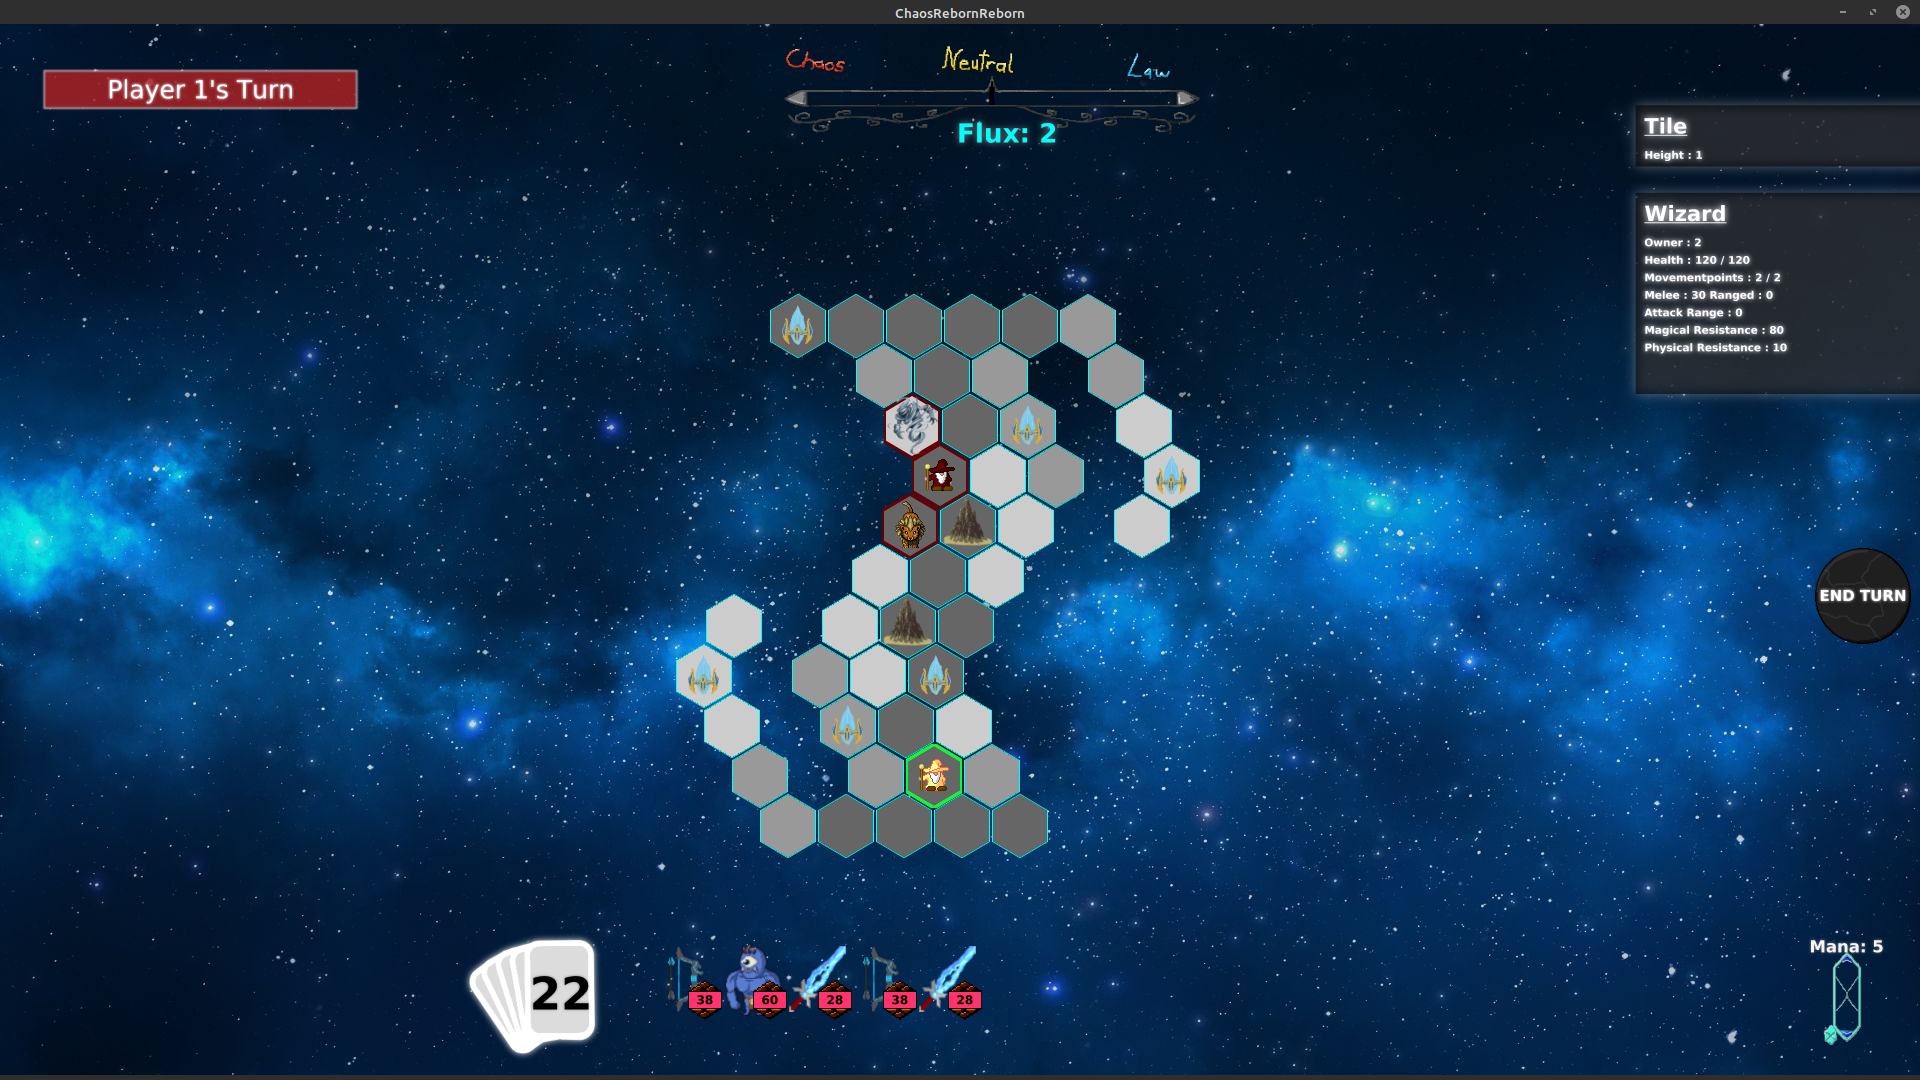
\includegraphics[width=\textwidth]{Prog2_EA_V2/screenshots/Anwendung4.png}\end{center}
	Mit einem Klick auf den \glqq END TURN\grqq Button wird die Runde von Spieler 1 beendet und Spieler 2 ist am Zug. Spieler 2 tut es Spieler 1 gleich, bewegt sich und beschwört Kreaturen zur Hilfe gegen den Gegner.
	\begin{center}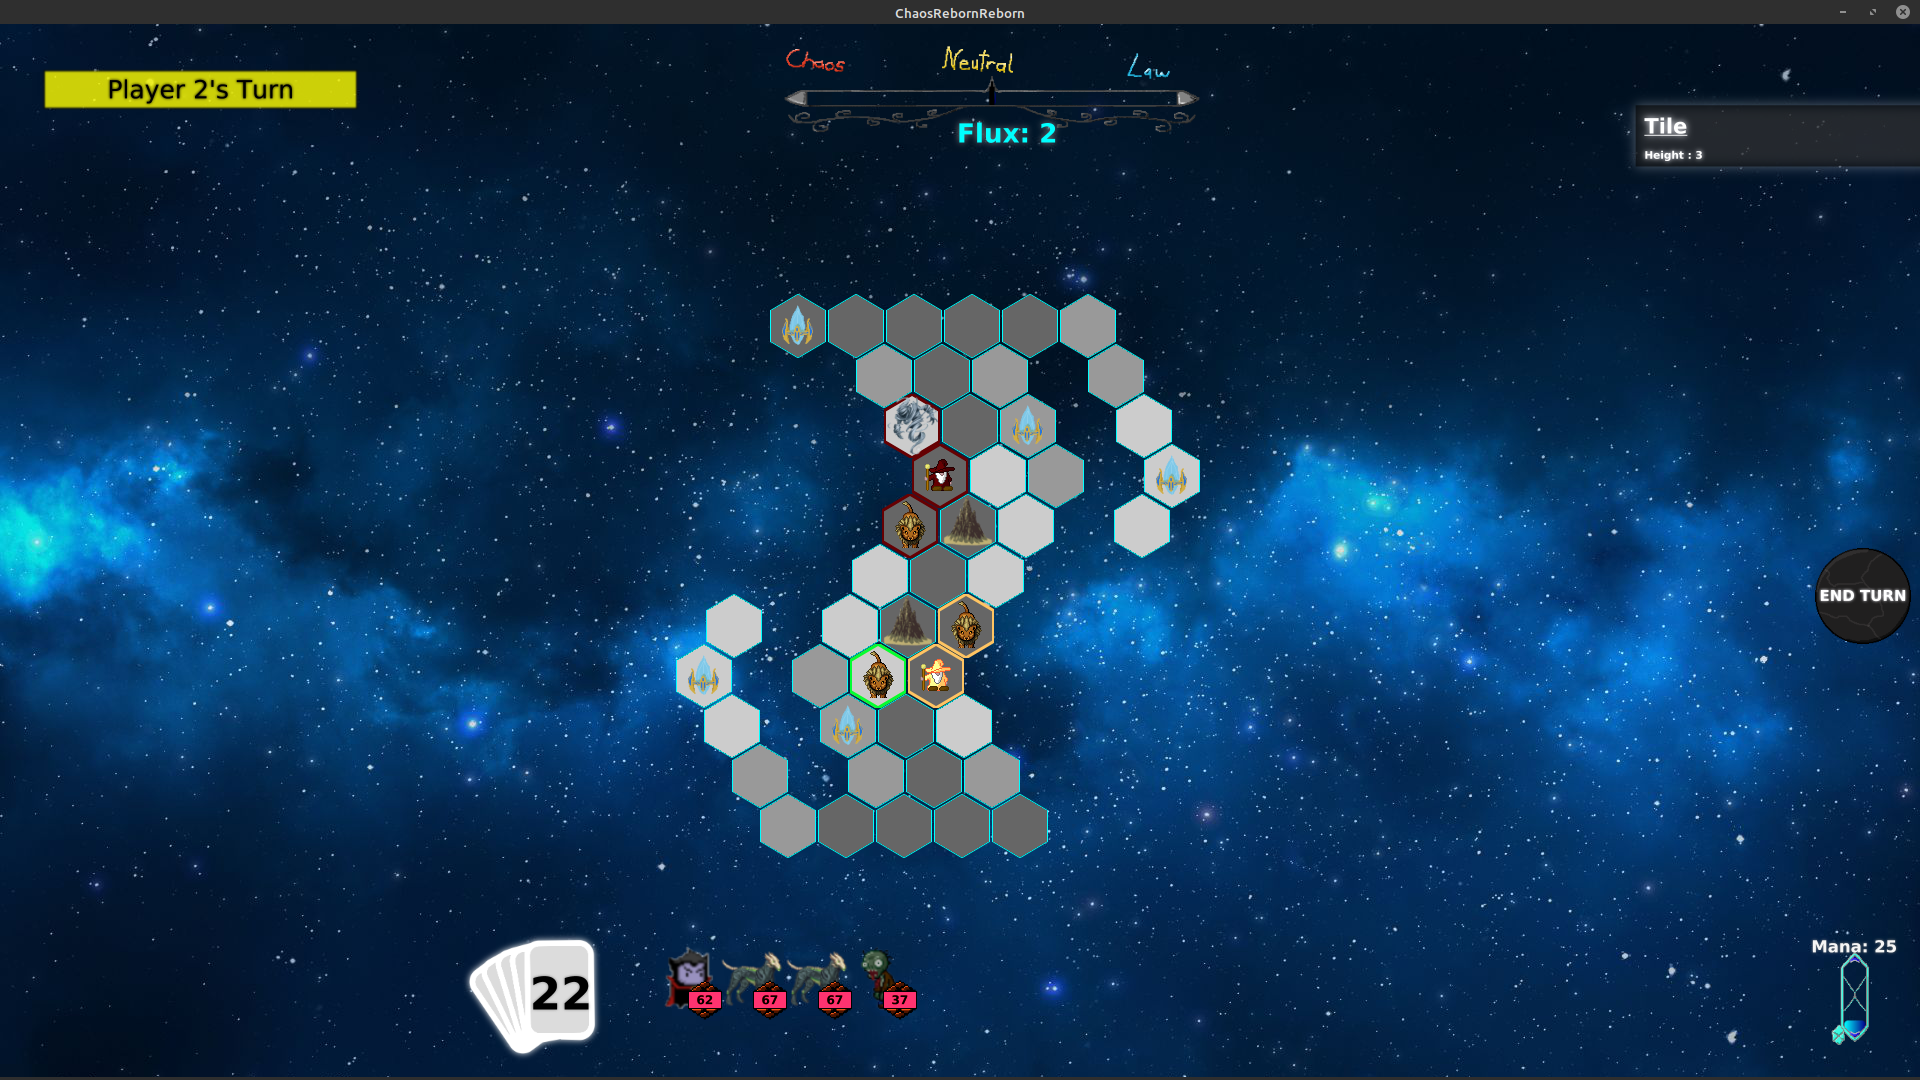
\includegraphics[width=\textwidth]{Prog2_EA_V2/screenshots/Anwendung5.png}\end{center}
	Spieler 1 bewegt daraufhin seine Kreaturen in Richtung des Gegners und greift mit dem eigenen den gegnerischen Löwen an.
	\begin{center}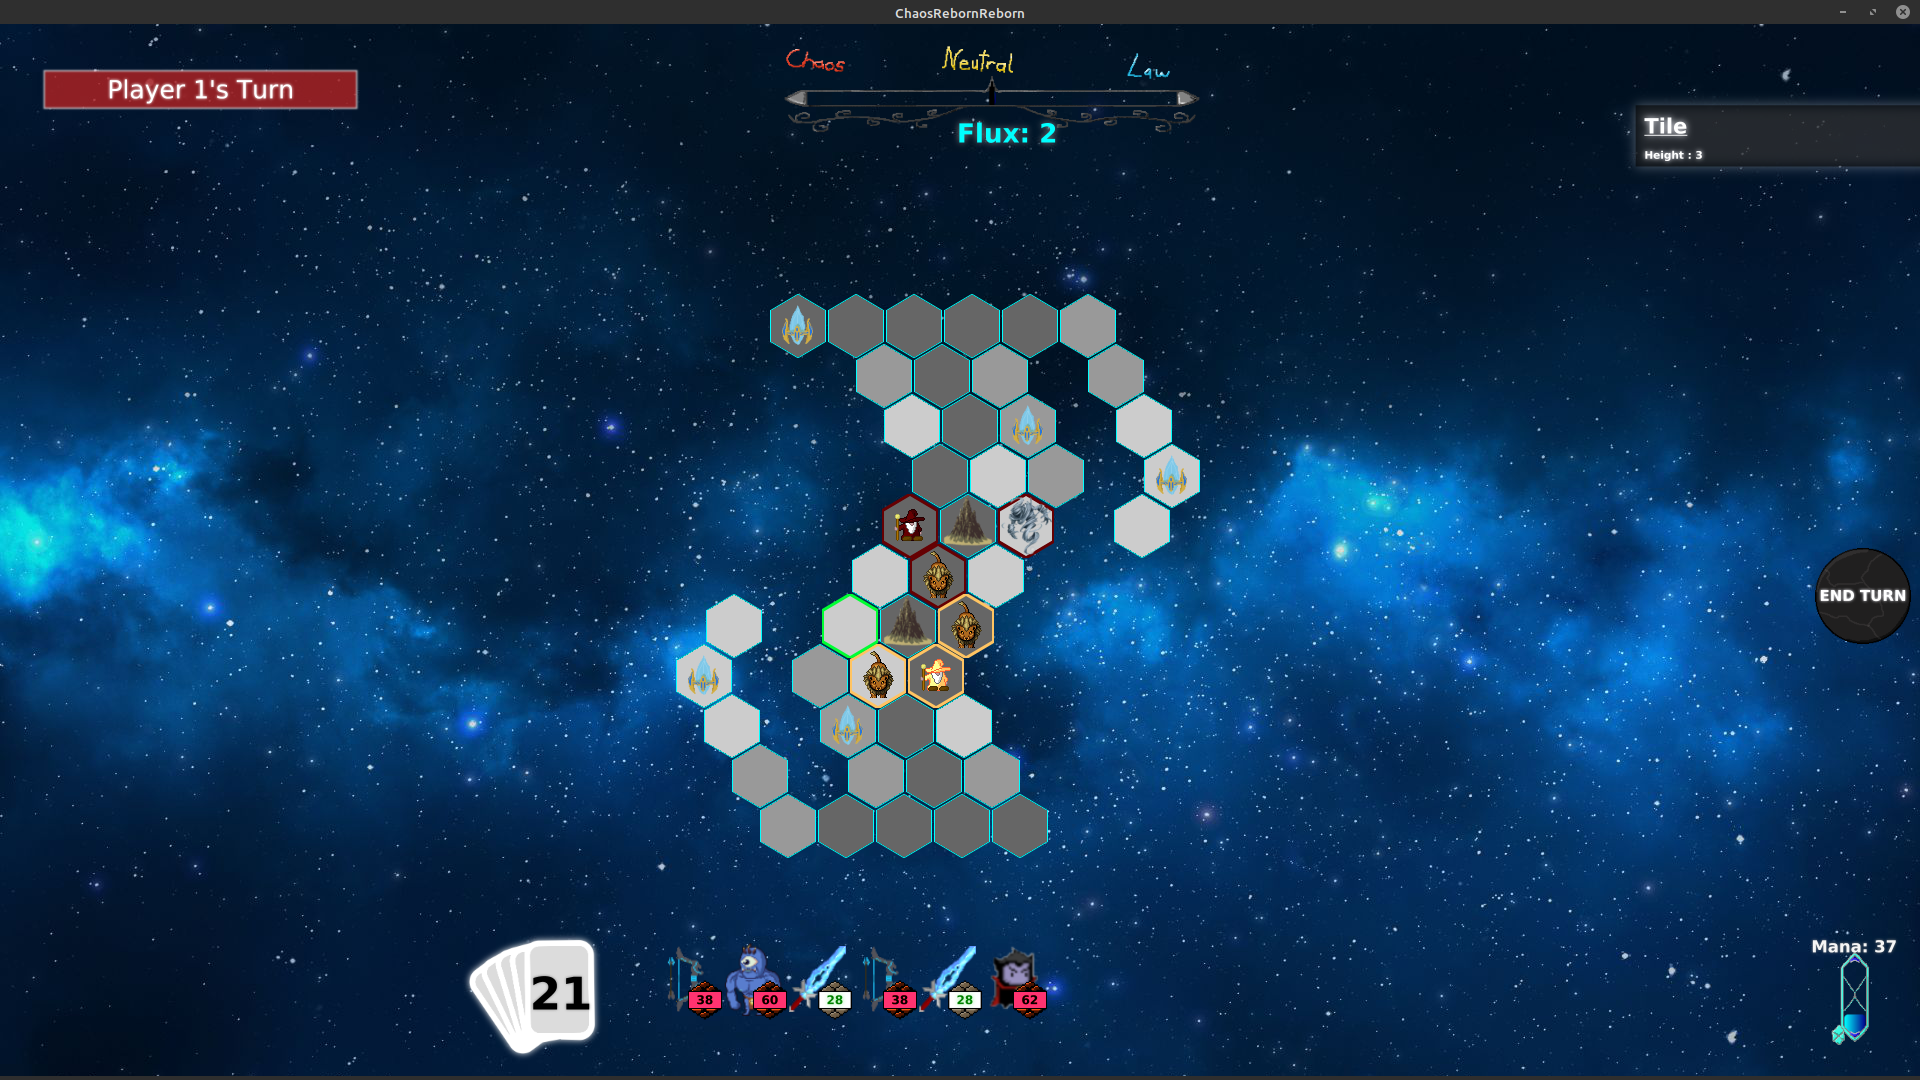
\includegraphics[width=\textwidth]{Prog2_EA_V2/screenshots/Anwendung6.png}\end{center}
	Weitere Kreaturen werden von den Zauberern beschworen und kämpfen gegeneinander. 
	\begin{center}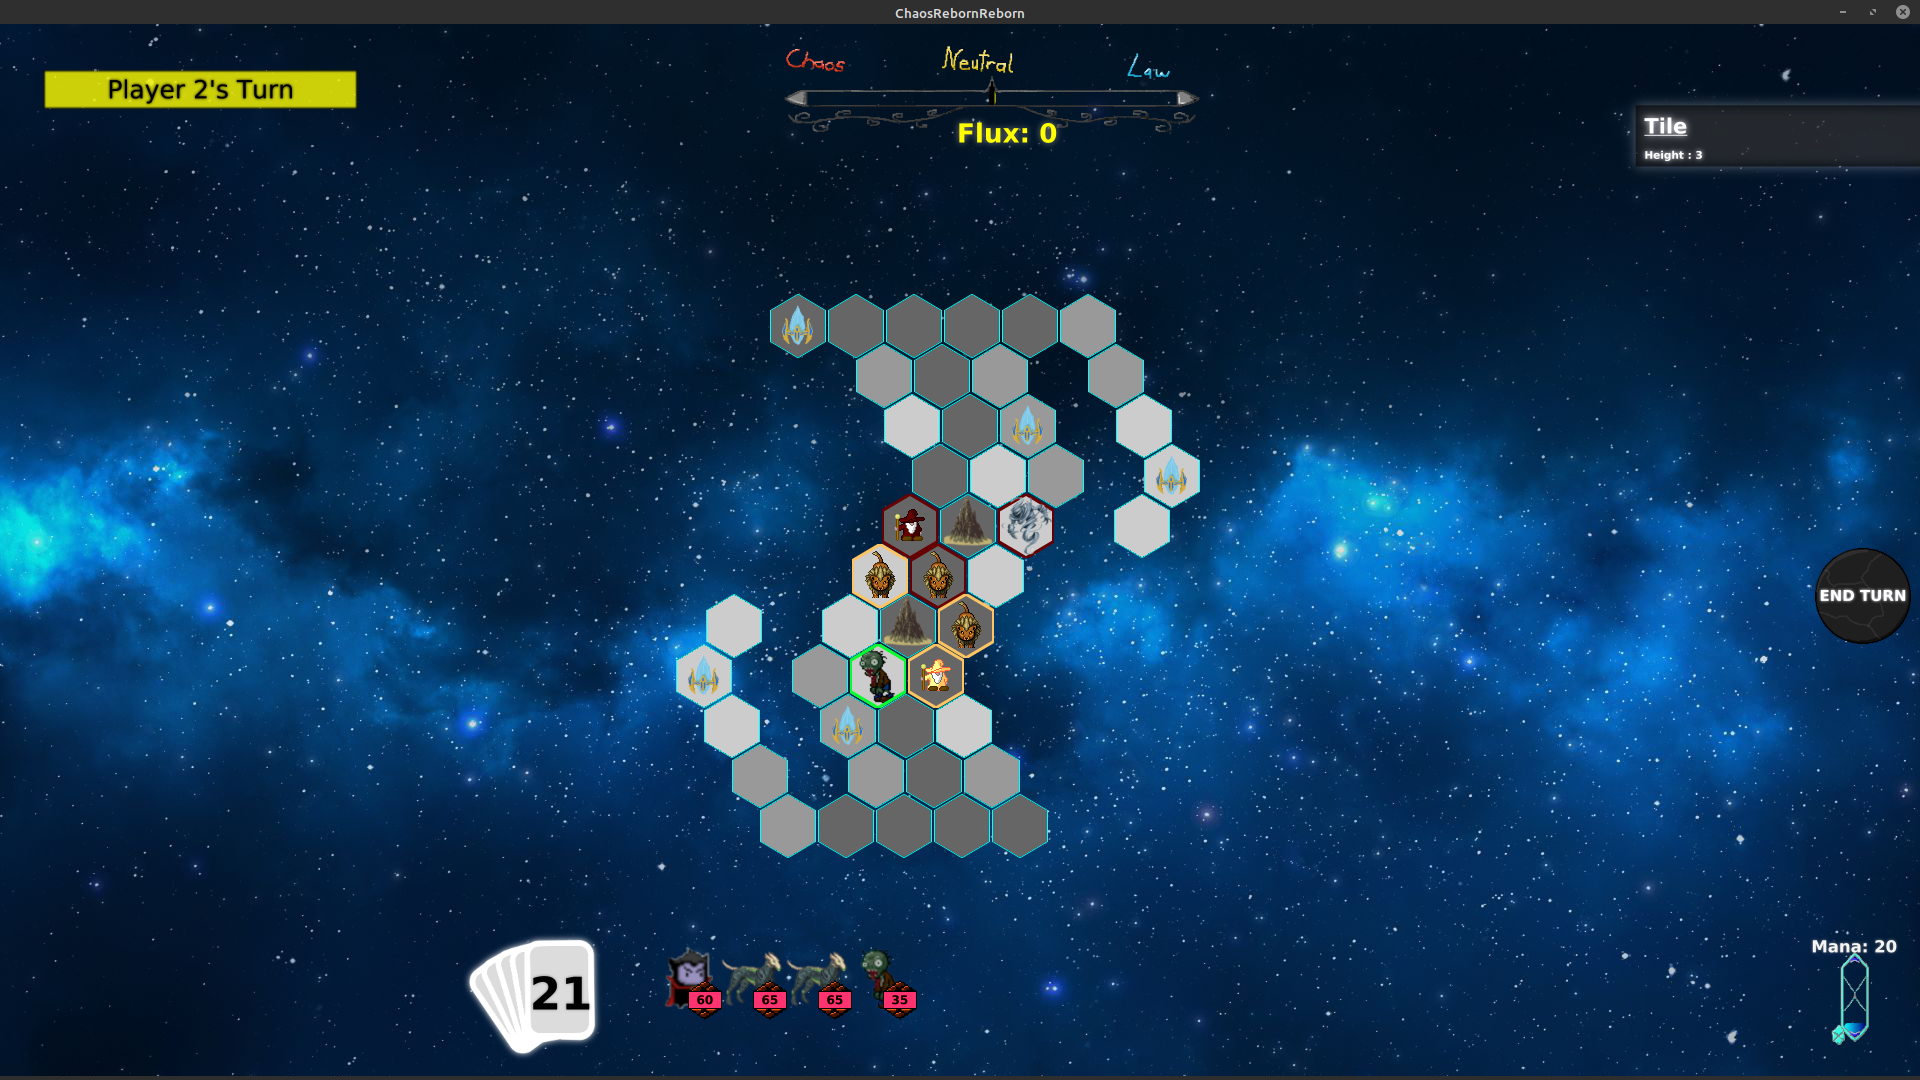
\includegraphics[width=\textwidth]{Prog2_EA_V2/screenshots/Anwendung7.png}\end{center}
	Nach langem Kämpfen der beiden Zauberer hat Spieler 1 Spieler 2 besiegt
	\begin{center}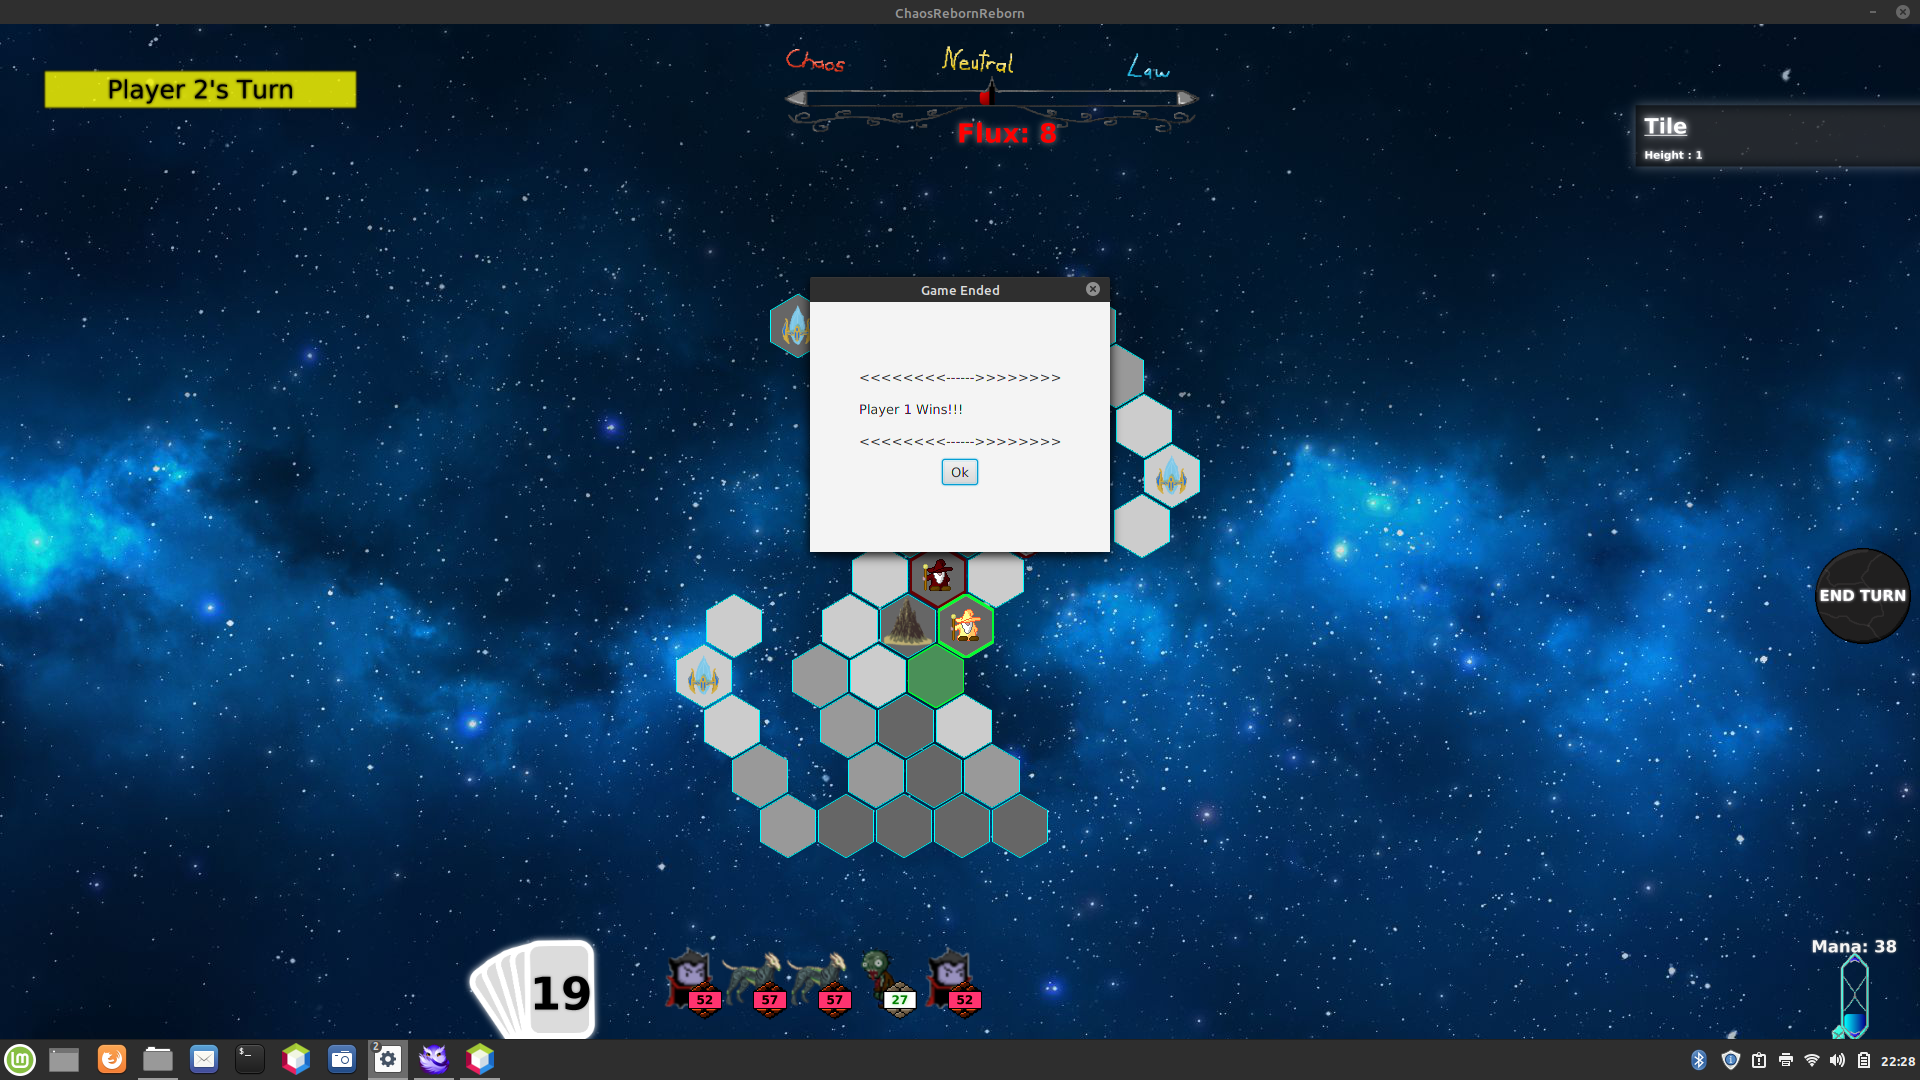
\includegraphics[width=\textwidth]{Prog2_EA_V2/screenshots/Anwendung8.png}\end{center}
	\newpage
	\section{Quelldateien}
	
	\subsection{Control}
	\subsubsection{Main.java}
	\lstinputlisting
	[caption={Main.java}
	\label{lst:javaclass},
	captionpos=t,language=JAVA,]
	{Prog2_EA_V2/src/Control/Main.java}
	\subsubsection{Game.java}
	\lstinputlisting
	[caption={Game.java}
	\label{lst:javaclass},
	captionpos=t,language=JAVA,]
	{Prog2_EA_V2/src/Control/Game.java}
	\subsection{Control.Actions}
	\subsubsection{Action}
	\lstinputlisting
	[caption={Action.java}
	\label{lst:javaclass},
	captionpos=t,language=JAVA,]
	{Prog2_EA_V2/src/Control/Actions/Action.java}
	\subsubsection{AttackAction}
	\lstinputlisting
	[caption={AttackAction.java}
	\label{lst:javaclass},
	captionpos=t,language=JAVA,]
	{Prog2_EA_V2/src/Control/Actions/AttackAction.java}
	\subsubsection{AttackMoveAction}
	\lstinputlisting
	[caption={AttackMoveAction.java}
	\label{lst:javaclass},
	captionpos=t,language=JAVA,]
	{Prog2_EA_V2/src/Control/Actions/AttackMoveAction.java}
	\subsubsection{ManaPickupAction}
	\lstinputlisting
	[caption={ManaPickupAction.java}
	\label{lst:javaclass},
	captionpos=t,language=JAVA,]
	{Prog2_EA_V2/src/Control/Actions/ManaPickupAction.java}
	\subsubsection{ManaPickupMoveAction}
	\lstinputlisting
	[caption={ManaPickupMoveAction.java}
	\label{lst:javaclass},
	captionpos=t,language=JAVA,]
	{Prog2_EA_V2/src/Control/Actions/ManaPickupMoveAction.java}
	\subsubsection{MeleeAttackAction}
	\lstinputlisting
	[caption={MeleeAttackAction.java}
	\label{lst:javaclass},
	captionpos=t,language=JAVA,]
	{Prog2_EA_V2/src/Control/Actions/MeleeAttackAction.java}
	\subsubsection{MoveAction}
	\lstinputlisting
	[caption={MoveAction.java}
	\label{lst:javaclass},
	captionpos=t,language=JAVA,]
	{Prog2_EA_V2/src/Control/Actions/MoveAction.java}
	\subsubsection{RangedAttackAction}
	\lstinputlisting
	[caption={RangedAttackAction.java}
	\label{lst:javaclass},
	captionpos=t,language=JAVA,]
	{Prog2_EA_V2/src/Control/Actions/RangedAttackAction.java}
	\subsection{Control.Controllers}
	\subsubsection{AnimationController}
	\lstinputlisting
	[caption={AnimationController.java}
	\label{lst:javaclass},
	captionpos=t,language=JAVA,]
	{Prog2_EA_V2/src/Control/Controllers/AnimationController.java}
	\subsubsection{GameController}
	\lstinputlisting
	[caption={GameController.java}
	\label{lst:javaclass},
	captionpos=t,language=JAVA,]
	{Prog2_EA_V2/src/Control/Controllers/GameController.java}
	\subsubsection{InputController}
	\lstinputlisting
	[caption={InputController.java}
	\label{lst:javaclass},
	captionpos=t,language=JAVA,]
	{Prog2_EA_V2/src/Control/Controllers/InputController.java}
	\subsubsection{MapController}
	\lstinputlisting
	[caption={MapController.java}
	\label{lst:javaclass},
	captionpos=t,language=JAVA,]
	{Prog2_EA_V2/src/Control/Controllers/MapController.java}
	\subsubsection{PlayerController}
	\lstinputlisting
	[caption={PlayerController.java}
	\label{lst:javaclass},
	captionpos=t,language=JAVA,]
	{Prog2_EA_V2/src/Control/Controllers/PlayerController.java}
	\subsubsection{SceneController}
	\lstinputlisting
	[caption={SceneController.java}
	\label{lst:javaclass},
	captionpos=t,language=JAVA,]
	{Prog2_EA_V2/src/Control/Controllers/SceneController.java}
	\subsubsection{SoundController}
	\lstinputlisting
	[caption={SoundController.java}
	\label{lst:javaclass},
	captionpos=t,language=JAVA,]
	{Prog2_EA_V2/src/Control/Controllers/SoundController.java}
	\subsubsection{TurnController}
	\lstinputlisting
	[caption={TurnController.java}
	\label{lst:javaclass},
	captionpos=t,language=JAVA,]
	{Prog2_EA_V2/src/Control/Controllers/TurnController.java}
	\subsection{Control.Network}
	\subsubsection{GameClient}
	\lstinputlisting
	[caption={GameClient.java}
	\label{lst:javaclass},
	captionpos=t,language=JAVA,]
	{Prog2_EA_V2/src/Control/Network/GameClient.java}
	\subsubsection{GameServer}
	\lstinputlisting
	[caption={GameServer.java}
	\label{lst:javaclass},
	captionpos=t,language=JAVA,]
	{Prog2_EA_V2/src/Control/Network/GameServer.java}
	\subsubsection{RecieveThread}
	\lstinputlisting
	[caption={RecieveThread.java}
	\label{lst:javaclass},
	captionpos=t,language=JAVA,]
	{Prog2_EA_V2/src/Control/Network/RecieveThread.java}
	\subsubsection{SendThread}
	\lstinputlisting
	[caption={SendThread.java}
	\label{lst:javaclass},
	captionpos=t,language=JAVA,]
	{Prog2_EA_V2/src/Control/Network/SendThread.java}
	\subsubsection{UserThread}
	\lstinputlisting
	[caption={UserThread.java}
	\label{lst:javaclass},
	captionpos=t,language=JAVA,]
	{Prog2_EA_V2/src/Control/Network/UserThread.java}
	\subsection{Control.Networks.Packets}
	\subsubsection{Packet}
	\lstinputlisting
	[caption={Packet.java}
	\label{lst:javaclass},
	captionpos=t,language=JAVA,]
	{Prog2_EA_V2/src/Control/Network/Packets/Packet.java}
	\subsubsection{PacketDecoder}
	\lstinputlisting
	[caption={PacketDecoder.java}
	\label{lst:javaclass},
	captionpos=t,language=JAVA,]
	{Prog2_EA_V2/src/Control/Network/Packets/PacketDecoder.java}
	\subsubsection{PacketType}
	\lstinputlisting
	[caption={PacketType.java}
	\label{lst:javaclass},
	captionpos=t,language=JAVA,]
	{Prog2_EA_V2/src/Control/Network/Packets/PacketType.java}
	\subsection{Control.SemiControllers}
	\subsubsection{Highlighter}
	\lstinputlisting
	[caption={Highlighter.java}
	\label{lst:javaclass},
	captionpos=t,language=JAVA,]
	{Prog2_EA_V2/src/Control/SemiControllers/Highlighter.java}
	\subsubsection{Selector}
	\lstinputlisting
	[caption={Selector.java}
	\label{lst:javaclass},
	captionpos=t,language=JAVA,]
	{Prog2_EA_V2/src/Control/SemiControllers/Selector.java}
	\subsection{Exceptions}
	\subsubsection{MapInvalidException}
	\lstinputlisting
	[caption={MapInvalidException.java}
	\label{lst:javaclass},
	captionpos=t,language=JAVA,]
	{Prog2_EA_V2/src/Exceptions/MapInvalidException.java}
	\subsubsection{MapTypeNotSupportedException}
	\lstinputlisting
	[caption={MapTypeNotSupportedException.java}
	\label{lst:javaclass},
	captionpos=t,language=JAVA,]
	{Prog2_EA_V2/src/Exceptions/MapTypeNotSupportedException.java}
	\subsubsection{UnexpectedCardException}
	\lstinputlisting
	[caption={UnexpectedCardException.java}
	\label{lst:javaclass},
	captionpos=t,language=JAVA,]
	{Prog2_EA_V2/src/Exceptions/UnexpectedCardException.java}
	\subsubsection{UnexpectedGameObjectException}
	\lstinputlisting
	[caption={.java}
	\label{lst:javaclass},
	captionpos=t,language=JAVA,]
	{Prog2_EA_V2/src/Exceptions/UnexpectedGameObjectException.java}
	\subsection{Model}
	\subsubsection{Player}
	\lstinputlisting
	[caption={Player.java}
	\label{lst:javaclass},
	captionpos=t,language=JAVA,]
	{Prog2_EA_V2/src/Model/Player.java}
	\subsection{Model.Card}
	\subsubsection{CardAdapter}
	\lstinputlisting
	[caption={CardAdapter.java}
	\label{lst:javaclass},
	captionpos=t,language=JAVA,]
	{Prog2_EA_V2/src/Model/Card/CardAdapter.java}
	\subsubsection{CardEffectAdapter}
	\lstinputlisting
	[caption={CardEffectAdapter.java}
	\label{lst:javaclass},
	captionpos=t,language=JAVA,]
	{Prog2_EA_V2/src/Model/Card/CardEffectAdapter.java}
	\subsubsection{CardStack}
	\lstinputlisting
	[caption={CardStack.java}
	\label{lst:javaclass},
	captionpos=t,language=JAVA,]
	{Prog2_EA_V2/src/Model/Card/CardStack.java}
	\subsubsection{CardType}
	\lstinputlisting
	[caption={CardType.java}
	\label{lst:javaclass},
	captionpos=t,language=JAVA,]
	{Prog2_EA_V2/src/Model/Card/CardType.java}
	\subsubsection{Deck}
	\lstinputlisting
	[caption={Deck.java}
	\label{lst:javaclass},
	captionpos=t,language=JAVA,]
	{Prog2_EA_V2/src/Model/Card/Deck.java}
	\subsubsection{EffectTag}
	\lstinputlisting
	[caption={EffectTag.java}
	\label{lst:javaclass},
	captionpos=t,language=JAVA,]
	{Prog2_EA_V2/src/Model/Card/EffectTag.java}
	\subsubsection{GenericCardEffect}
	\lstinputlisting
	[caption={GenericCardEffect.java}
	\label{lst:javaclass},
	captionpos=t,language=JAVA,]
	{Prog2_EA_V2/src/Model/Card/GenericCardEffect.java}
	\subsubsection{Hand}
	\lstinputlisting
	[caption={Hand.java}
	\label{lst:javaclass},
	captionpos=t,language=JAVA,]
	{Prog2_EA_V2/src/Model/Card/Hand.java}
	\subsubsection{ICard}
	\lstinputlisting
	[caption={ICard.java}
	\label{lst:javaclass},
	captionpos=t,language=JAVA,]
	{Prog2_EA_V2/src/Model/Card/ICard.java}
	\subsubsection{ICardEffect}
	\lstinputlisting
	[caption={ICardEffect.java}
	\label{lst:javaclass},
	captionpos=t,language=JAVA,]
	{Prog2_EA_V2/src/Model/Card/ICardEffect.java}
	\subsubsection{Wand}
	\lstinputlisting
	[caption={Wand.java}
	\label{lst:javaclass},
	captionpos=t,language=JAVA,]
	{Prog2_EA_V2/src/Model/Card/Wand.java}
	\subsubsection{WandFactory}
	\lstinputlisting
	[caption={WandFactory.java}
	\label{lst:javaclass},
	captionpos=t,language=JAVA,]
	{Prog2_EA_V2/src/Model/Card/WandFactory.java}
	\subsection{Model.Card.AllCards}
	\subsubsection{CardFactory}
	\lstinputlisting
	[caption={CardFactory.java}
	\label{lst:javaclass},
	captionpos=t,language=JAVA,]
	{Prog2_EA_V2/src/Model/Card/AllCards/CardFactory.java}
	\subsection{Model.Card.AllCards.Spells}
	\subsubsection{AttackSpell}
	\lstinputlisting
	[caption={AttackSpell.java}
	\label{lst:javaclass},
	captionpos=t,language=JAVA,]
	{Prog2_EA_V2/src/Model/Card/AllCards/Spells/AttackSpell.java}
	\subsubsection{Spell}
	\lstinputlisting
	[caption={Spell.java}
	\label{lst:javaclass},
	captionpos=t,language=JAVA,]
	{Prog2_EA_V2/src/Model/Card/AllCards/Spells/Spell.java}
	\subsection{Model.Card.AllCards.Spells.Chaos}
	\subsubsection{Vengeance}
	\lstinputlisting
	[caption={Vengeance.java}
	\label{lst:javaclass},
	captionpos=t,language=JAVA,]
	{Prog2_EA_V2/src/Model/Card/AllCards/Spells/Chaos/Vengeance.java}
	\subsection{Model.Card.AllCards.Spells.Law}
	\subsubsection{Decree}
	\lstinputlisting
	[caption={Decree.java}
	\label{lst:javaclass},
	captionpos=t,language=JAVA,]
	{Prog2_EA_V2/src/Model/Card/AllCards/Spells/Law/Decree.java}
	\subsubsection{DivineBow}
	\lstinputlisting
	[caption={DivineBow.java}
	\label{lst:javaclass},
	captionpos=t,language=JAVA,]
	{Prog2_EA_V2/src/Model/Card/AllCards/Spells/Law/DivineBow.java}
	\subsubsection{DivineShield}
	\lstinputlisting
	[caption={DivineShield.java}
	\label{lst:javaclass},
	captionpos=t,language=JAVA,]
	{Prog2_EA_V2/src/Model/Card/AllCards/Spells/Law/DivineShield.java}
	\subsubsection{DivineSword}
	\lstinputlisting
	[caption={DivineSword.java}
	\label{lst:javaclass},
	captionpos=t,language=JAVA,]
	{Prog2_EA_V2/src/Model/Card/AllCards/Spells/Law/DivineSword.java}
	\subsection{Model.Card.AllCards.Spells.Neutral}
	\subsubsection{MagicBolt}
	\lstinputlisting
	[caption={MagicBolt.java}
	\label{lst:javaclass},
	captionpos=t,language=JAVA,]
	{Prog2_EA_V2/src/Model/Card/AllCards/Spells/Neutral/MagicBolt.java}
	\subsubsection{WindWalker}
	\lstinputlisting
	[caption={WindWalker.java}
	\label{lst:javaclass},
	captionpos=t,language=JAVA,]
	{Prog2_EA_V2/src/Model/Card/AllCards/Spells/Neutral/WindWalker.java}
	\subsection{Model.Card.AllCards.Summons}
	\subsubsection{Summon}
	\lstinputlisting
	[caption={Summon.java}
	\label{lst:javaclass},
	captionpos=t,language=JAVA,]
	{Prog2_EA_V2/src/Model/Card/AllCards/Summons/Summon.java}
	\subsubsection{SummonEffect}
	\lstinputlisting
	[caption={SummonEffect.java}
	\label{lst:javaclass},
	captionpos=t,language=JAVA,]
	{Prog2_EA_V2/src/Model/Card/AllCards/Summons/SummonEffect.java}
	\subsection{Model.Card.AllCards.Summons.Chaos}
	\subsubsection{Hellhound}
	\lstinputlisting
	[caption={Hellhound.java}
	\label{lst:javaclass},
	captionpos=t,language=JAVA,]
	{Prog2_EA_V2/src/Model/Card/AllCards/Summons/Chaos/Hellhound.java}
	\subsubsection{Hydra}
	\lstinputlisting
	[caption={Hydra.java}
	\label{lst:javaclass},
	captionpos=t,language=JAVA,]
	{Prog2_EA_V2/src/Model/Card/AllCards/Summons/Chaos/Hydra.java}
	\subsubsection{Manticore}
	\lstinputlisting
	[caption={Manticore.java}
	\label{lst:javaclass},
	captionpos=t,language=JAVA,]
	{Prog2_EA_V2/src/Model/Card/AllCards/Summons/Chaos/Manticore.java}
	\subsubsection{Skeleton}
	\lstinputlisting
	[caption={Skeleton.java}
	\label{lst:javaclass},
	captionpos=t,language=JAVA,]
	{Prog2_EA_V2/src/Model/Card/AllCards/Summons/Chaos/Skeleton.java}
	\subsubsection{Vampire}
	\lstinputlisting
	[caption={Vampire.java}
	\label{lst:javaclass},
	captionpos=t,language=JAVA,]
	{Prog2_EA_V2/src/Model/Card/AllCards/Summons/Chaos/Vampire.java}
	\subsubsection{Zombie}
	\lstinputlisting
	[caption={Zombie.java}
	\label{lst:javaclass},
	captionpos=t,language=JAVA,]
	{Prog2_EA_V2/src/Model/Card/AllCards/Summons/Chaos/Zombie.java}
	\subsection{Model.Card.AllCards.Summons.Law}
	\subsubsection{IcarusTower}
	\lstinputlisting
	[caption={IcarusTower.java}
	\label{lst:javaclass},
	captionpos=t,language=JAVA,]
	{Prog2_EA_V2/src/Model/Card/AllCards/Summons/Law/IcarusTower.java}
	\subsubsection{Paladin}
	\lstinputlisting
	[caption={Paladin.java}
	\label{lst:javaclass},
	captionpos=t,language=JAVA,]
	{Prog2_EA_V2/src/Model/Card/AllCards/Summons/Law/Paladin.java}
	\subsubsection{Pegasus}
	\lstinputlisting
	[caption={Pegasus.java}
	\label{lst:javaclass},
	captionpos=t,language=JAVA,]
	{Prog2_EA_V2/src/Model/Card/AllCards/Summons/Law/Pegasus.java}
	\subsubsection{SapphireDragon}
	\lstinputlisting
	[caption={SapphireDragon.java}
	\label{lst:javaclass},
	captionpos=t,language=JAVA,]
	{Prog2_EA_V2/src/Model/Card/AllCards/Summons/Law/SapphireDragon.java}
	\subsection{Model.Card.AllCards.Summons.Neutral}
	\subsubsection{AirElemental}
	\lstinputlisting
	[caption={AirElemental.java}
	\label{lst:javaclass},
	captionpos=t,language=JAVA,]
	{Prog2_EA_V2/src/Model/Card/AllCards/Summons/Neutral/AirElemental.java}
	\subsubsection{Eagle}
	\lstinputlisting
	[caption={Eagle.java}
	\label{lst:javaclass},
	captionpos=t,language=JAVA,]
	{Prog2_EA_V2/src/Model/Card/AllCards/Summons/Neutral/Eagle.java}
	\subsubsection{Giant}
	\lstinputlisting
	[caption={Giant.java}
	\label{lst:javaclass},
	captionpos=t,language=JAVA,]
	{Prog2_EA_V2/src/Model/Card/AllCards/Summons/Neutral/Giant.java}
	\subsubsection{Lion}
	\lstinputlisting
	[caption={Lion.java}
	\label{lst:javaclass},
	captionpos=t,language=JAVA,]
	{Prog2_EA_V2/src/Model/Card/AllCards/Summons/Neutral/Lion.java}
	\subsection{Model.Card.Wands}
	\subsubsection{AirWand}
	\lstinputlisting
	[caption={AirWand.java}
	\label{lst:javaclass},
	captionpos=t,language=JAVA,]
	{Prog2_EA_V2/src/Model/Card/Wands/AirWand.java}
	\subsubsection{CreatureWand}
	\lstinputlisting
	[caption={CreatureWand.java}
	\label{lst:javaclass},
	captionpos=t,language=JAVA,]
	{Prog2_EA_V2/src/Model/Card/Wands/CreatureWand.java}
	\subsubsection{RandomWand}
	\lstinputlisting
	[caption={RandomWand.java}
	\label{lst:javaclass},
	captionpos=t,language=JAVA,]
	{Prog2_EA_V2/src/Model/Card/Wands/RandomWand.java}
	\subsubsection{UndeadWand}
	\lstinputlisting
	[caption={UndeadWand.java}
	\label{lst:javaclass},
	captionpos=t,language=JAVA,]
	{Prog2_EA_V2/src/Model/Card/Wands/UndeadWand.java}
	\subsection{Model.Game}
	\subsubsection{FluxMeter}
	\lstinputlisting
	[caption={FluxMeter.java}
	\label{lst:javaclass},
	captionpos=t,language=JAVA,]
	{Prog2_EA_V2/src/Model/Game/FluxMeter.java}
	\subsection{Model.GameObject}
	\subsubsection{Attribute}
	\lstinputlisting
	[caption={Attribute.java}
	\label{lst:javaclass},
	captionpos=t,language=JAVA,]
	{Prog2_EA_V2/src/Model/GameObject/Attribute.java}
	\subsubsection{CreatureAdapter}
	\lstinputlisting
	[caption={CreatureAdapter.java}
	\label{lst:javaclass},
	captionpos=t,language=JAVA,]
	{Prog2_EA_V2/src/Model/GameObject/CreatureAdapter.java}
	\subsubsection{GameObject}
	\lstinputlisting
	[caption={GameObject.java}
	\label{lst:javaclass},
	captionpos=t,language=JAVA,]
	{Prog2_EA_V2/src/Model/GameObject/GameObject.java}
	\subsubsection{GameObjects}
	\lstinputlisting
	[caption={GameObjects.java}
	\label{lst:javaclass},
	captionpos=t,language=JAVA,]
	{Prog2_EA_V2/src/Model/GameObject/GameObjects.java}
	\subsubsection{IAttackable}
	\lstinputlisting
	[caption={IAttackable.java}
	\label{lst:javaclass},
	captionpos=t,language=JAVA,]
	{Prog2_EA_V2/src/Model/GameObject/IAttackable.java}
	\subsubsection{ManaCrystal}
	\lstinputlisting
	[caption={ManaCrystal.java}
	\label{lst:javaclass},
	captionpos=t,language=JAVA,]
	{Prog2_EA_V2/src/Model/GameObject/ManaCrystal.java}
	\subsubsection{Obstacle}
	\lstinputlisting
	[caption={Obstacle.java}
	\label{lst:javaclass},
	captionpos=t,language=JAVA,]
	{Prog2_EA_V2/src/Model/GameObject/Obstacle.java}
	\subsubsection{PlayerCharacter}
	\lstinputlisting
	[caption={PlayerCharacter.java}
	\label{lst:javaclass},
	captionpos=t,language=JAVA,]
	{Prog2_EA_V2/src/Model/GameObject/PlayerCharacter.java}
	\subsubsection{SummonableMinion}
	\lstinputlisting
	[caption={SummonableMinion.java}
	\label{lst:javaclass},
	captionpos=t,language=JAVA,]
	{Prog2_EA_V2/src/Model/GameObject/SummonableMinion.java}
	\subsection{Model.GameObject.Minions.Chaos}
	\subsubsection{HellhoundMinion}
	\lstinputlisting
	[caption={HellhoundMinion.java}
	\label{lst:javaclass},
	captionpos=t,language=JAVA,]
	{Prog2_EA_V2/src/Model/GameObject/Minions/Chaos/HellhoundMinion.java}
	\subsubsection{HydraMinion}
	\lstinputlisting
	[caption={HydraMinion.java}
	\label{lst:javaclass},
	captionpos=t,language=JAVA,]
	{Prog2_EA_V2/src/Model/GameObject/Minions/Chaos/HydraMinion.java}
	\subsubsection{ManticoreMinion}
	\lstinputlisting
	[caption={ManticoreMinion.java}
	\label{lst:javaclass},
	captionpos=t,language=JAVA,]
	{Prog2_EA_V2/src/Model/GameObject/Minions/Chaos/ManticoreMinion.java}
	\subsubsection{SkeletonMinion}
	\lstinputlisting
	[caption={ManticoreMinion.java}
	\label{lst:javaclass},
	captionpos=t,language=JAVA,]
	{Prog2_EA_V2/src/Model/GameObject/Minions/Chaos/ManticoreMinion.java}
	\subsubsection{VampireMinion}
	\lstinputlisting
	[caption={VampireMinion.java}
	\label{lst:javaclass},
	captionpos=t,language=JAVA,]
	{Prog2_EA_V2/src/Model/GameObject/Minions/Chaos/VampireMinion.java}
	\subsubsection{ZombieMinion}
	\lstinputlisting
	[caption={ZombieMinion.java}
	\label{lst:javaclass},
	captionpos=t,language=JAVA,]
	{Prog2_EA_V2/src/Model/GameObject/Minions/Chaos/ZombieMinion.java}
	\subsection{Model.GameObject.Minions.Law}
	\subsubsection{IcarusTowerMinion}
	\lstinputlisting
	[caption={GameIcarusTowerMinion.java}
	\label{lst:javaclass},
	captionpos=t,language=JAVA,]
	{Prog2_EA_V2/src/Model/GameObject/Minions/Law/IcarusTowerMinion.java}
	\subsubsection{PaladinMinion}
	\lstinputlisting
	[caption={PaladinMinion.java}
	\label{lst:javaclass},
	captionpos=t,language=JAVA,]
	{Prog2_EA_V2/src/Model/GameObject/Minions/Law/PaladinMinion.java}
	\subsubsection{PegasusMinion}
	\lstinputlisting
	[caption={PegasusMinion.java}
	\label{lst:javaclass},
	captionpos=t,language=JAVA,]
	{Prog2_EA_V2/src/Model/GameObject/Minions/Law/PegasusMinion.java}
	\subsubsection{SapphireDragonMinion}
	\lstinputlisting
	[caption={SapphireDragonMinion.java}
	\label{lst:javaclass},
	captionpos=t,language=JAVA,]
	{Prog2_EA_V2/src/Model/GameObject/Minions/Law/SapphireDragonMinion.java}
	\subsection{Model.GameObject.Minions.Neutral}
	\subsubsection{AirElementalMinion}
	\lstinputlisting
	[caption={AirElementalMinion.java}
	\label{lst:javaclass},
	captionpos=t,language=JAVA,]
	{Prog2_EA_V2/src/Model/GameObject/Minions/Neutral/AirElementalMinion.java}
	\subsubsection{EagleMinion}
	\lstinputlisting
	[caption={EagleMinion.java}
	\label{lst:javaclass},
	captionpos=t,language=JAVA,]
	{Prog2_EA_V2/src/Model/GameObject/Minions/Neutral/EagleMinion.java}
	\subsubsection{GiantMinion}
	\lstinputlisting
	[caption={GiantMinion.java}
	\label{lst:javaclass},
	captionpos=t,language=JAVA,]
	{Prog2_EA_V2/src/Model/GameObject/Minions/Neutral/GiantMinion.java}
	\subsubsection{LionMinion}
	\lstinputlisting
	[caption={LionMinion.java}
	\label{lst:javaclass},
	captionpos=t,language=JAVA,]
	{Prog2_EA_V2/src/Model/GameObject/Minions/Neutral/LionMinion.java}
	\subsection{Model.Map}
	\subsubsection{AxialTransform}
	\lstinputlisting
	[caption={AxialTransform.java}
	\label{lst:javaclass},
	captionpos=t,language=JAVA,]
	{Prog2_EA_V2/src/Model/Map/AxialTransform.java}
	\subsubsection{CubeTransform}
	\lstinputlisting
	[caption={CubeTransform.java}
	\label{lst:javaclass},
	captionpos=t,language=JAVA,]
	{Prog2_EA_V2/src/Model/Map/CubeTransform.java}
	\subsubsection{FloatCubeTransform}
	\lstinputlisting
	[caption={FloatCubeTransform.java}
	\label{lst:javaclass},
	captionpos=t,language=JAVA,]
	{Prog2_EA_V2/src/Model/Map/FloatCubeTransform.java}
	\subsubsection{Map}
	\lstinputlisting
	[caption={Map.java}
	\label{lst:javaclass},
	captionpos=t,language=JAVA,]
	{Prog2_EA_V2/src/Model/Map/Map.java}
	\subsubsection{MapGenArgs}
	\lstinputlisting
	[caption={MapGenArgs.java}
	\label{lst:javaclass},
	captionpos=t,language=JAVA,]
	{Prog2_EA_V2/src/Model/Map/MapGenArgs.java}
	\subsubsection{MapGenerationKeywords}
	\lstinputlisting
	[caption={MapGenerationKeywords.java}
	\label{lst:javaclass},
	captionpos=t,language=JAVA,]
	{Prog2_EA_V2/src/Model/Map/MapGenerationKeywords.java}
	\subsubsection{MapGenerator}
	\lstinputlisting
	[caption={MapGenerator.java}
	\label{lst:javaclass},
	captionpos=t,language=JAVA,]
	{Prog2_EA_V2/src/Model/Map/MapGenerator.java}
	\subsubsection{Pathfinding}
	\lstinputlisting
	[caption={Pathfinding.java}
	\label{lst:javaclass},
	captionpos=t,language=JAVA,]
	{Prog2_EA_V2/src/Model/Map/Pathfinding.java}
	\subsubsection{PerlinNoise}
	\lstinputlisting
	[caption={PerlinNoise.java}
	\label{lst:javaclass},
	captionpos=t,language=JAVA,]
	{Prog2_EA_V2/src/Model/Map/PerlinNoise.java}
	\subsubsection{Tile}
	\lstinputlisting
	[caption={Tile.java}
	\label{lst:javaclass},
	captionpos=t,language=JAVA,]
	{Prog2_EA_V2/src/Model/Map/Tile.java}
	\subsection{Resource}
	\subsubsection{Dimensions}
	\lstinputlisting
	[caption={Dimensions.java}
	\label{lst:javaclass},
	captionpos=t,language=JAVA,]
	{Prog2_EA_V2/src/Resource/Dimensions.java}
	\subsubsection{VideoOptions}
	\lstinputlisting
	[caption={VideoOptions.java}
	\label{lst:javaclass},
	captionpos=t,language=JAVA,]
	{Prog2_EA_V2/src/Resource/VideoOptions.java}
	\subsection{Resource.Constants.CardConstants}
	\subsubsection{CardConstants}
	\lstinputlisting
	[caption={CardConstants.java}
	\label{lst:javaclass},
	captionpos=t,language=JAVA,]
	{Prog2_EA_V2/src/Resource/Constants/CardConstants/CardConstants.java}
	\subsection{Resource.Constants.CardConstants.SpellConstants.Chaos}
	\subsubsection{VengeanceSpellConstants}
	\lstinputlisting
	[caption={VengeanceSpellConstants.java}
	\label{lst:javaclass},
	captionpos=t,language=JAVA,]
	{Prog2_EA_V2/src/Resource/Constants/CardConstants/SpellConstants/Chaos/VengeanceSpellConstants.java}
	\subsection{Resource.Constants.CardConstants.SpellConstants.Law}
	\subsubsection{DecreeSpellConstants}
	\lstinputlisting
	[caption={DecreeSpellConstants.java}
	\label{lst:javaclass},
	captionpos=t,language=JAVA,]
	{Prog2_EA_V2/src/Resource/Constants/CardConstants/SpellConstants/Law/DecreeSpellConstants.java}
	\subsubsection{DivineBowSpellConstants}
	\lstinputlisting
	[caption={DivineBowSpellConstants.java}
	\label{lst:javaclass},
	captionpos=t,language=JAVA,]
	{Prog2_EA_V2/src/Resource/Constants/CardConstants/SpellConstants/Law/DivineBowSpellConstants.java}
	\subsubsection{DivineShieldSpellConstants}
	\lstinputlisting
	[caption={DivineShieldSpellConstants.java}
	\label{lst:javaclass},
	captionpos=t,language=JAVA,]
	{Prog2_EA_V2/src/Resource/Constants/CardConstants/SpellConstants/Law/DivineShieldSpellConstants.java}
	\subsubsection{DivineSwordSpellConstants}
	\lstinputlisting
	[caption={DivineSwordSpellConstants.java}
	\label{lst:javaclass},
	captionpos=t,language=JAVA,]
	{Prog2_EA_V2/src/Resource/Constants/CardConstants/SpellConstants/Law/DivineSwordSpellConstants.java}
	\subsection{Resource.Constants.CardConstants.SpellConstants.Neutral}
	\subsubsection{MagicBoltSpellConstants}
	\lstinputlisting
	[caption={MagicBoltSpellConstants.java}
	\label{lst:javaclass},
	captionpos=t,language=JAVA,]
	{Prog2_EA_V2/src/Resource/Constants/CardConstants/SpellConstants/Neutral/MagicBoltSpellConstants.java}
	\subsubsection{WindWalkerSpellConstants}
	\lstinputlisting
	[caption={WindWalkerSpellConstants.java}
	\label{lst:javaclass},
	captionpos=t,language=JAVA,]
	{Prog2_EA_V2/src/Resource/Constants/CardConstants/SpellConstants/Neutral/WindWalkerSpellConstants.java}
	\subsection{Resource.Constants.CardConstants.SummonConstants}
	\subsubsection{SummonConstants}
	\lstinputlisting
	[caption={SummonConstants.java}
	\label{lst:javaclass},
	captionpos=t,language=JAVA,]
	{Prog2_EA_V2/src/Resource/Constants/CardConstants/SummonConstants/SummonConstants.java}
	\subsection{Resource.Constants.CardConstants.SummonConstants.Chaos}
	\subsubsection{HellhoundSummonConstants}
	\lstinputlisting
	[caption={HellhoundSummonConstants.java}
	\label{lst:javaclass},
	captionpos=t,language=JAVA,]
	{Prog2_EA_V2/src/Resource/Constants/CardConstants/SummonConstants/Chaos/HellhoundSummonConstants.java}
	\subsubsection{HydraSummonConstants}
	\lstinputlisting
	[caption={HydraSummonConstants.java}
	\label{lst:javaclass},
	captionpos=t,language=JAVA,]
	{Prog2_EA_V2/src/Resource/Constants/CardConstants/SummonConstants/Chaos/HydraSummonConstants.java}
	\subsubsection{ManticoreSummonConstants}
	\lstinputlisting
	[caption={ManticoreSummonConstants.java}
	\label{lst:javaclass},
	captionpos=t,language=JAVA,]
	{Prog2_EA_V2/src/Resource/Constants/CardConstants/SummonConstants/Chaos/ManticoreSummonConstants.java}
	\subsubsection{SkeletonSummonConstants}
	\lstinputlisting
	[caption={SkeletonSummonConstants.java}
	\label{lst:javaclass},
	captionpos=t,language=JAVA,]
	{Prog2_EA_V2/src/Resource/Constants/CardConstants/SummonConstants/Chaos/SkeletonSummonConstants.java}
	\subsubsection{VampireSummonConstants}
	\lstinputlisting
	[caption={VampireSummonConstants.java}
	\label{lst:javaclass},
	captionpos=t,language=JAVA,]
	{Prog2_EA_V2/src/Resource/Constants/CardConstants/SummonConstants/Chaos/VampireSummonConstants.java}
	\subsubsection{ZombieSummonConstants}
	\lstinputlisting
	[caption={ZombieSummonConstants.java}
	\label{lst:javaclass},
	captionpos=t,language=JAVA,]
	{Prog2_EA_V2/src/Resource/Constants/CardConstants/SummonConstants/Chaos/ZombieSummonConstants.java}
	\subsection{Resource.Constants.CardConstants.Law}
	\subsubsection{IcarusTowerSummonConstants}
	\lstinputlisting
	[caption={IcarusTowerSummonConstants.java}
	\label{lst:javaclass},
	captionpos=t,language=JAVA,]
	{Prog2_EA_V2/src/Resource/Constants/CardConstants/SummonConstants/Law/IcarusTowerSummonConstants.java}
	\subsubsection{PaladinSummonConstants}
	\lstinputlisting
	[caption={PaladinSummonConstants.java}
	\label{lst:javaclass},
	captionpos=t,language=JAVA,]
	{Prog2_EA_V2/src/Resource/Constants/CardConstants/SummonConstants/Law/PaladinSummonConstants.java}
	\subsubsection{PegasusSummonConstants}
	\lstinputlisting
	[caption={PegasusSummonConstants.java}
	\label{lst:javaclass},
	captionpos=t,language=JAVA,]
	{Prog2_EA_V2/src/Resource/Constants/CardConstants/SummonConstants/Law/PegasusSummonConstants.java}
	\subsubsection{SapphireDragonSummonConstants}
	\lstinputlisting
	[caption={SapphireDragonSummonConstants.java}
	\label{lst:javaclass},
	captionpos=t,language=JAVA,]
	{Prog2_EA_V2/src/Resource/Constants/CardConstants/SummonConstants/Law/SapphireDragonSummonConstants.java}
	\subsection{Resource.Constants.CardConstants.Neutral}
	\subsubsection{AirElementalSummonConstants}
	\lstinputlisting
	[caption={AirElementalSummonConstants.java}
	\label{lst:javaclass},
	captionpos=t,language=JAVA,]
	{Prog2_EA_V2/src/Resource/Constants/CardConstants/SummonConstants/Neutral/AirElementalSummonConstants.java}
	\subsubsection{EagleSummonConstants}
	\lstinputlisting
	[caption={EagleSummonConstants.java}
	\label{lst:javaclass},
	captionpos=t,language=JAVA,]
	{Prog2_EA_V2/src/Resource/Constants/CardConstants/SummonConstants/Neutral/EagleSummonConstants.java}
	\subsubsection{GiantSummonConstants}
	\lstinputlisting
	[caption={GiantSummonConstants.java}
	\label{lst:javaclass},
	captionpos=t,language=JAVA,]
	{Prog2_EA_V2/src/Resource/Constants/CardConstants/SummonConstants/Neutral/GiantSummonConstants.java}
	\subsubsection{LionSummonConstants}
	\lstinputlisting
	[caption={LionSummonConstants.java}
	\label{lst:javaclass},
	captionpos=t,language=JAVA,]
	{Prog2_EA_V2/src/Resource/Constants/CardConstants/SummonConstants/Neutral/LionSummonConstants.java}
	\subsection{Resource.Constants.CardConstants.WandConstants}
	\subsubsection{AirWandConstants}
	\lstinputlisting
	[caption={AirWandConstants.java}
	\label{lst:javaclass},
	captionpos=t,language=JAVA,]
	{Prog2_EA_V2/src/Resource/Constants/CardConstants/WandConstants/AirWandConstants.java}
	\subsubsection{CreatureWandConstants}
	\lstinputlisting
	[caption={CreatureWandConstants.java}
	\label{lst:javaclass},
	captionpos=t,language=JAVA,]
	{Prog2_EA_V2/src/Resource/Constants/CardConstants/WandConstants/CreatureWandConstants.java}
	\subsubsection{RandomWandConstants}
	\lstinputlisting
	[caption={RandomWandConstants.java}
	\label{lst:javaclass},
	captionpos=t,language=JAVA,]
	{Prog2_EA_V2/src/Resource/Constants/CardConstants/WandConstants/RandomWandConstants.java}
	\subsubsection{UndeadWandConstants}
	\lstinputlisting
	[caption={UndeadWandConstants.java}
	\label{lst:javaclass},
	captionpos=t,language=JAVA,]
	{Prog2_EA_V2/src/Resource/Constants/CardConstants/WandConstants/UndeadWandConstants.java}
	\subsection{Resource.Constants.GeneralConstants}
    \subsubsection{ActionConstants}
	\lstinputlisting
	[caption={ActionConstants.java}
	\label{lst:javaclass},
	captionpos=t,language=JAVA,]
	{Prog2_EA_V2/src/Resource/Constants/GeneralConstants/ActionConstants.java}
	\subsubsection{ControllerConstants}
	\lstinputlisting
	[caption={ControllerConstants.java}
	\label{lst:javaclass},
	captionpos=t,language=JAVA,]
	{Prog2_EA_V2/src/Resource/Constants/GeneralConstants/ControllerConstants.java}
	\subsubsection{GameConstants}
	\lstinputlisting
	[caption={GameConstants.java}
	\label{lst:javaclass},
	captionpos=t,language=JAVA,]
	{Prog2_EA_V2/src/Resource/Constants/GeneralConstants/GameConstants.java}
	\subsubsection{GameObjectConstants}
	\lstinputlisting
	[caption={GameObjectConstants.java}
	\label{lst:javaclass},
	captionpos=t,language=JAVA,]
	{Prog2_EA_V2/src/Resource/Constants/GeneralConstants/GameObjectConstants.java}
	\subsubsection{MapConstants}
	\lstinputlisting
	[caption={MapConstants.java}
	\label{lst:javaclass},
	captionpos=t,language=JAVA,]
	{Prog2_EA_V2/src/Resource/Constants/GeneralConstants/MapConstants.java}
	\subsubsection{MenuConstants}
	\lstinputlisting
	[caption={MenuConstants.java}
	\label{lst:javaclass},
	captionpos=t,language=JAVA,]
	{Prog2_EA_V2/src/Resource/Constants/GeneralConstants/MenuConstants.java}
	\subsubsection{NetworkConstants}
	\lstinputlisting
	[caption={NetworkConstants.java}
	\label{lst:javaclass},
	captionpos=t,language=JAVA,]
	{Prog2_EA_V2/src/Resource/Constants/GeneralConstants/NetworkConstants.java}
	\subsubsection{PlayerConstants}
	\lstinputlisting
	[caption={PlayerConstants.java}
	\label{lst:javaclass},
	captionpos=t,language=JAVA,]
	{Prog2_EA_V2/src/Resource/Constants/GeneralConstants/PlayerConstants.java}
    \subsubsection{PopUpConstants}
	\lstinputlisting
	[caption={PopUpConstants.java}
	\label{lst:javaclass},
	captionpos=t,language=JAVA,]
	{Prog2_EA_V2/src/Resource/Constants/GeneralConstants/PopUpConstants.java}
	\subsubsection{SoundConstants}
	\lstinputlisting
	[caption={SoundConstants.java}
	\label{lst:javaclass},
	captionpos=t,language=JAVA,]
	{Prog2_EA_V2/src/Resource/Constants/GeneralConstants/SoundConstants.java}
	\subsubsection{UIConstants}
	\lstinputlisting
	[caption={UIConstants.java}
	\label{lst:javaclass},
	captionpos=t,language=JAVA,]
	{Prog2_EA_V2/src/Resource/Constants/GeneralConstants/UIConstants.java}
	\subsection{Resource.Constants.MinionConstants}
	\subsubsection{PlayerCharacterMinionConstants}
	\lstinputlisting
	[caption={PlayerCharacterMinionConstants.java}
	\label{lst:javaclass},
	captionpos=t,language=JAVA,]
	{Prog2_EA_V2/src/Resource/Constants/MinionConstants/PlayerCharacterMinionConstants.java}
	\subsection{Resource.Constants.MinionConstants.Chaos}
	\subsubsection{HellhoundMinionConstants}
	\lstinputlisting
	[caption={HellhoundMinionConstants.java}
	\label{lst:javaclass},
	captionpos=t,language=JAVA,]
	{Prog2_EA_V2/src/Resource/Constants/MinionConstants/Chaos/HellhoundMinionConstants.java}
	\subsubsection{HydraMinionConstants}
	\lstinputlisting
	[caption={HydraMinionConstants.java}
	\label{lst:javaclass},
	captionpos=t,language=JAVA,]
	{Prog2_EA_V2/src/Resource/Constants/MinionConstants/Chaos/HydraMinionConstants.java}
	\subsubsection{ManticoreMinionConstants}
	\lstinputlisting
	[caption={ManticoreMinionConstants.java}
	\label{lst:javaclass},
	captionpos=t,language=JAVA,]
	{Prog2_EA_V2/src/Resource/Constants/MinionConstants/Chaos/ManticoreMinionConstants.java}
	\subsubsection{SkeletonMinionConstants}
	\lstinputlisting
	[caption={SkeletonMinionConstants.java}
	\label{lst:javaclass},
	captionpos=t,language=JAVA,]
	{Prog2_EA_V2/src/Resource/Constants/MinionConstants/Chaos/SkeletonMinionConstants.java}
	\subsubsection{VampireMinionConstants}
	\lstinputlisting
	[caption={VampireMinionConstants.java}
	\label{lst:javaclass},
	captionpos=t,language=JAVA,]
	{Prog2_EA_V2/src/Resource/Constants/MinionConstants/Chaos/VampireMinionConstants.java}
	\subsubsection{ZombieMinionConstants}
	\lstinputlisting
	[caption={ZombieMinionConstants.java}
	\label{lst:javaclass},
	captionpos=t,language=JAVA,]
	{Prog2_EA_V2/src/Resource/Constants/MinionConstants/Chaos/ZombieMinionConstants.java}
	\subsection{Resource.Constants.MinionConstants.Law}
	\subsubsection{IcarusTowerMinionConstants}
	\lstinputlisting
	[caption={IcarusTowerMinionConstants.java}
	\label{lst:javaclass},
	captionpos=t,language=JAVA,]
	{Prog2_EA_V2/src/Resource/Constants/MinionConstants/Law/IcarusTowerMinionConstants.java}
	\subsubsection{PaladinMinionConstants}
	\lstinputlisting
	[caption={PaladinMinionConstants.java}
	\label{lst:javaclass},
	captionpos=t,language=JAVA,]
	{Prog2_EA_V2/src/Resource/Constants/MinionConstants/Law/PaladinMinionConstants.java}
	\subsubsection{PegasusMinionConstants}
	\lstinputlisting
	[caption={PegasusMinionConstants.java}
	\label{lst:javaclass},
	captionpos=t,language=JAVA,]
	{Prog2_EA_V2/src/Resource/Constants/MinionConstants/Law/PegasusMinionConstants.java}
	\subsubsection{SapphireDragonMinionConstants}
	\lstinputlisting
	[caption={SapphireDragonMinionConstants.java}
	\label{lst:javaclass},
	captionpos=t,language=JAVA,]
	{Prog2_EA_V2/src/Resource/Constants/MinionConstants/Law/SapphireDragonMinionConstants.java}
	\subsection{Resource.Constants.MinionConstants.Neutral}
	\subsubsection{AirElementalMinionConstants}
	\lstinputlisting
	[caption={AirElementalMinionConstants.java}
	\label{lst:javaclass},
	captionpos=t,language=JAVA,]
	{Prog2_EA_V2/src/Resource/Constants/MinionConstants/Neutral/AirElementalMinionConstants.java}
	\subsubsection{EagleMinionConstants}
	\lstinputlisting
	[caption={EagleMinionConstants.java}
	\label{lst:javaclass},
	captionpos=t,language=JAVA,]
	{Prog2_EA_V2/src/Resource/Constants/MinionConstants/Neutral/EagleMinionConstants.java}
	\subsubsection{GiantMinionConstants}
	\lstinputlisting
	[caption={GiantMinionConstants.java}
	\label{lst:javaclass},
	captionpos=t,language=JAVA,]
	{Prog2_EA_V2/src/Resource/Constants/MinionConstants/Neutral/GiantMinionConstants.java}
	\subsubsection{LionMinionConstants}
	\lstinputlisting
	[caption={LionMinionConstants.java}
	\label{lst:javaclass},
	captionpos=t,language=JAVA,]
	{Prog2_EA_V2/src/Resource/Constants/MinionConstants/Neutral/LionMinionConstants.java}
	\subsection{Resource.Images}
	\subsubsection{Animations}
	\lstinputlisting
	[caption={Animations.java}
	\label{lst:javaclass},
	captionpos=t,language=JAVA,]
	{Prog2_EA_V2/src/Resource/Images/Animations.java}
	\subsubsection{CardExclusiveImages}
	\lstinputlisting
	[caption={CardExclusiveImages.java}
	\label{lst:javaclass},
	captionpos=t,language=JAVA,]
	{Prog2_EA_V2/src/Resource/Images/CardExclusiveImages.java}
	\subsubsection{GOImages}
	\lstinputlisting
	[caption={GOImages.java}
	\label{lst:javaclass},
	captionpos=t,language=JAVA,]
	{Prog2_EA_V2/src/Resource/Images/GOImages.java}
	\subsubsection{HexImages}
	\lstinputlisting
	[caption={HexImages.java}
	\label{lst:javaclass},
	captionpos=t,language=JAVA,]
	{Prog2_EA_V2/src/Resource/Images/HexImages.java}
	\subsubsection{Images}
	\lstinputlisting
	[caption={Images.java}
	\label{lst:javaclass},
	captionpos=t,language=JAVA,]
	{Prog2_EA_V2/src/Resource/Images/Images.java}
	\subsubsection{UIElementsImages}
	\lstinputlisting
	[caption={UIElementsImages.java}
	\label{lst:javaclass},
	captionpos=t,language=JAVA,]
	{Prog2_EA_V2/src/Resource/Images/UIElementImages.java}
	\subsubsection{WandImages}
	\lstinputlisting
	[caption={WandImages.java}
	\label{lst:javaclass},
	captionpos=t,language=JAVA,]
	{Prog2_EA_V2/src/Resource/Images/WandImages.java}
	\subsection{Util}
	\subsubsection{Stack}
	\lstinputlisting
	[caption={Stack.java}
	\label{lst:javaclass},
	captionpos=t,language=JAVA,]
	{Prog2_EA_V2/src/Util/Stack.java}
	\subsection{View.Menus}
	\subsubsection{MainMenu}
	\lstinputlisting
	[caption={MainMenu.java}
	\label{lst:javaclass},
	captionpos=t,language=JAVA,]
	{Prog2_EA_V2/src/View/Menus/MainMenu.java}
	\subsubsection{MapOptionsMenu}
	\lstinputlisting
	[caption={MapOptionsMenu.java}
	\label{lst:javaclass},
	captionpos=t,language=JAVA,]
	{Prog2_EA_V2/src/View/Menus/MapOptionsMenu.java}
	\subsubsection{Menu}
	\lstinputlisting
	[caption={Menu.java}
	\label{lst:javaclass},
	captionpos=t,language=JAVA,]
	{Prog2_EA_V2/src/View/Menus/Menu.java}
	\subsubsection{MultiplayerMenu}
	\lstinputlisting
	[caption={MultiplayerMenu.java}
	\label{lst:javaclass},
	captionpos=t,language=JAVA,]
	{Prog2_EA_V2/src/View/Menus/MultiplayerMenu.java}
	\subsubsection{OptionsMenu}
	\lstinputlisting
	[caption={OptionsMenu.java}
	\label{lst:javaclass},
	captionpos=t,language=JAVA,]
	{Prog2_EA_V2/src/View/Menus/OptionsMenu.java}
	\subsubsection{PauseMenu}
	\lstinputlisting
	[caption={PauseMenu.java}
	\label{lst:javaclass},
	captionpos=t,language=JAVA,]
	{Prog2_EA_V2/src/View/Menus/PauseMenu.java}
	\subsubsection{SoundMenu}
	\lstinputlisting
	[caption={SoundMenu.java}
	\label{lst:javaclass},
	captionpos=t,language=JAVA,]
	{Prog2_EA_V2/src/View/Menus/SoundMenu.java}
	\subsection{View.PopUps}
	\subsubsection{ConnectionPopUp}
	\lstinputlisting
	[caption={ConnectionPopUp.java}
	\label{lst:javaclass},
	captionpos=t,language=JAVA,]
	{Prog2_EA_V2/src/View/PopUps/ConnectionPopUp.java}
	\subsubsection{MapSavePopUp}
	\lstinputlisting
	[caption={MapSavePopUp.java}
	\label{lst:javaclass},
	captionpos=t,language=JAVA,]
	{Prog2_EA_V2/src/View/PopUps/MapSavePopUp.java}
	\subsubsection{PopUp}
	\lstinputlisting
	[caption={PopUp.java}
	\label{lst:javaclass},
	captionpos=t,language=JAVA,]
	{Prog2_EA_V2/src/View/PopUps/PopUp.java}
	\subsubsection{WinPopUp}
	\lstinputlisting
	[caption={WinPopUp.java}
	\label{lst:javaclass},
	captionpos=t,language=JAVA,]
	{Prog2_EA_V2/src/View/PopUps/WinPopUp.java}
	\subsection{View.Scenes}
	\subsubsection{ChaosScene}
	\lstinputlisting
	[caption={ChaosScene.java}
	\label{lst:javaclass},
	captionpos=t,language=JAVA,]
	{Prog2_EA_V2/src/View/Scenes/ChaosScene.java}
	\subsubsection{GameScene}
	\lstinputlisting
	[caption={GameScene.java}
	\label{lst:javaclass},
	captionpos=t,language=JAVA,]
	{Prog2_EA_V2/src/View/Scenes/GameScene.java}
	\subsubsection{GameSetupScene}
	\lstinputlisting
	[caption={GameSetupScene.java}
	\label{lst:javaclass},
	captionpos=t,language=JAVA,]
	{Prog2_EA_V2/src/View/Scenes/GameSetupScene.java}
	\subsubsection{GameSetupSceneMP}
	\lstinputlisting
	[caption={GameSetupSceneMP.java}
	\label{lst:javaclass},
	captionpos=t,language=JAVA,]
	{Prog2_EA_V2/src/View/Scenes/GameSetupSceneMP.java}
	\subsubsection{MenuScene}
	\lstinputlisting
	[caption={MenuScene.java}
	\label{lst:javaclass},
	captionpos=t,language=JAVA,]
	{Prog2_EA_V2/src/View/Scenes/MenuScene.java}
	\subsection{View.Stylesheets}
	\subsubsection{MenuButton}
	\lstinputlisting
	[caption={MenuButton.css}
	\label{lst:javaclass},
	captionpos=t,language=JAVA,]
	{Prog2_EA_V2/src/View/Stylesheets/MenuButton.css}
	\subsubsection{MenuItem}
	\lstinputlisting
	[caption={MenuItem.css}
	\label{lst:javaclass},
	captionpos=t,language=JAVA,]
	{Prog2_EA_V2/src/View/Stylesheets/MenuItem.css}
	\subsubsection{MenuSlider}
	\lstinputlisting
	[caption={MenuSlider.css}
	\label{lst:javaclass},
	captionpos=t,language=JAVA,]
	{Prog2_EA_V2/src/View/Stylesheets/MenuSlider.css}
	\subsubsection{MenuTextField}
	\lstinputlisting
	[caption={MenuTextField.css}
	\label{lst:javaclass},
	captionpos=t,language=JAVA,]
	{Prog2_EA_V2/src/View/Stylesheets/MenuTextField.css}
	\subsection{View.Tooltip}
	\subsubsection{CardTooltip}
	\lstinputlisting
	[caption={CardTooltip.java}
	\label{lst:javaclass},
	captionpos=t,language=JAVA,]
	{Prog2_EA_V2/src/View/Tooltip/CardTooltip.java}
	\subsubsection{GOTooltip}
	\lstinputlisting
	[caption={GOTooltip.java}
	\label{lst:javaclass},
	captionpos=t,language=JAVA,]
	{Prog2_EA_V2/src/View/Tooltip/GOTooltip.java}
	\subsubsection{MinionTooltip}
	\lstinputlisting
	[caption={MinionTooltip.java}
	\label{lst:javaclass},
	captionpos=t,language=JAVA,]
	{Prog2_EA_V2/src/View/Tooltip/MinionTooltip.java}
	\subsubsection{TileTooltip}
	\lstinputlisting
	[caption={TileTooltip.java}
	\label{lst:javaclass},
	captionpos=t,language=JAVA,]
	{Prog2_EA_V2/src/View/Tooltip/TileTooltip.java}
	\subsubsection{Tooltip}
	\lstinputlisting
	[caption={Tooltip.java}
	\label{lst:javaclass},
	captionpos=t,language=JAVA,]
	{Prog2_EA_V2/src/View/Tooltip/Tooltip.java}
	\subsubsection{TooltipBox}
	\lstinputlisting
	[caption={TooltipBox.java}
	\label{lst:javaclass},
	captionpos=t,language=JAVA,]
	{Prog2_EA_V2/src/View/Tooltip/TooltipBox.java}
	\subsubsection{WandTooltip}
	\lstinputlisting
	[caption={WandTooltip.java}
	\label{lst:javaclass},
	captionpos=t,language=JAVA,]
	{Prog2_EA_V2/src/View/Tooltip/WandTooltip.java}
	\subsection{View.UIElements}
	\subsubsection{CardView}
	\lstinputlisting
	[caption={CardView.java}
	\label{lst:javaclass},
	captionpos=t,language=JAVA,]
	{Prog2_EA_V2/src/View/UIElements/CardView.java}
	\subsubsection{ChaosBackground}
	\lstinputlisting
	[caption={ChaosBackground.java}
	\label{lst:javaclass},
	captionpos=t,language=JAVA,]
	{Prog2_EA_V2/src/View/UIElements/ChaosBackground.java}
	\subsubsection{ChaosMenuButton}
	\lstinputlisting
	[caption={ChaosMenuButton.java}
	\label{lst:javaclass},
	captionpos=t,language=JAVA,]
	{Prog2_EA_V2/src/View/UIElements/ChaosMenuButton.java}
	\subsubsection{ChaosVBox}
	\lstinputlisting
	[caption={ChaosVBox.java}
	\label{lst:javaclass},
	captionpos=t,language=JAVA,]
	{Prog2_EA_V2/src/View/UIElements/ChaosVBox.java}
	\subsubsection{DeckUI}
	\lstinputlisting
	[caption={DeckUI.java}
	\label{lst:javaclass},
	captionpos=t,language=JAVA,]
	{Prog2_EA_V2/src/View/UIElements/DeckUI.java}
	\subsubsection{FluxBar}
	\lstinputlisting
	[caption={FluxBar.java}
	\label{lst:javaclass},
	captionpos=t,language=JAVA,]
	{Prog2_EA_V2/src/View/UIElements/FluxBar.java}
	\subsubsection{HandView}
	\lstinputlisting
	[caption={HandView.java}
	\label{lst:javaclass},
	captionpos=t,language=JAVA,]
	{Prog2_EA_V2/src/View/UIElements/HandView.java}
	\subsubsection{IChaosUI}
	\lstinputlisting
	[caption={IChaosUI.java}
	\label{lst:javaclass},
	captionpos=t,language=JAVA,]
	{Prog2_EA_V2/src/View/UIElements/IChaosUI.java}
	\subsubsection{ManaBar}
	\lstinputlisting
	[caption={ManaBar.java}
	\label{lst:javaclass},
	captionpos=t,language=JAVA,]
	{Prog2_EA_V2/src/View/UIElements/ManaBar.java}
	\subsubsection{MapView}
	\lstinputlisting
	[caption={MapView.java}
	\label{lst:javaclass},
	captionpos=t,language=JAVA,]
	{Prog2_EA_V2/src/View/UIElements/MapView.java}
	\subsubsection{MusicAndEffect}
	\lstinputlisting
	[caption={MusicAndEffect.java}
	\label{lst:javaclass},
	captionpos=t,language=JAVA,]
	{Prog2_EA_V2/src/View/UIElements/MusicAndEffect.java}
	\subsubsection{PlayerWandView}
	\lstinputlisting
	[caption={PlayerWandView.java}
	\label{lst:javaclass},
	captionpos=t,language=JAVA,]
	{Prog2_EA_V2/src/View/UIElements/PlayerWandView.java}
	\subsubsection{RoundButton}
	\lstinputlisting
	[caption={RoundButton.java}
	\label{lst:javaclass},
	captionpos=t,language=JAVA,]
	{Prog2_EA_V2/src/View/UIElements/RoundButton.java}
	\subsubsection{TextWithBackground}
	\lstinputlisting
	[caption={TextWithBackground.java}
	\label{lst:javaclass},
	captionpos=t,language=JAVA,]
	{Prog2_EA_V2/src/View/UIElements/TextWithBackground.java}
	\subsubsection{TileView}
	\lstinputlisting
	[caption={TileView.java}
	\label{lst:javaclass},
	captionpos=t,language=JAVA,]
	{Prog2_EA_V2/src/View/UIElements/TileView.java}
	\subsubsection{TurnPlayerDisplay}
	\lstinputlisting
	[caption={TurnPlayerDisplay.java}
	\label{lst:javaclass},
	captionpos=t,language=JAVA,]
	{Prog2_EA_V2/src/View/UIElements/TurnPlayerDisplay.java}
	\subsubsection{WandView}
	\lstinputlisting
	[caption={WandView.java}
	\label{lst:javaclass},
	captionpos=t,language=JAVA,]
	{Prog2_EA_V2/src/View/UIElements/WandView.java}
	
	\section{Art}
	\subsection{AirElemental}
	\begin{center}
\includegraphics{Prog2_EA_V2/Art/AirElemental.png}\end{center}
	\subsection{AirWand}
	\begin{center}
\includegraphics{Prog2_EA_V2/Art/AirWand.png}\end{center}
	\subsection{BlueExplosion}
	\begin{center}
\includegraphics{Prog2_EA_V2/Art/BlueExplosion.png}\end{center}
	\subsection{Buff}
	\begin{center}
\includegraphics{Prog2_EA_V2/Art/Buff.png}\end{center}
	\subsection{CreatureWand}
	\begin{center}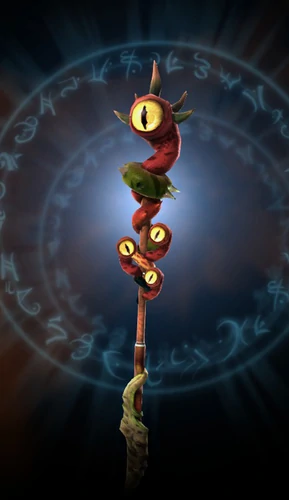
\includegraphics{Prog2_EA_V2/Art/CreatureWand.png}\end{center}
	\subsection{Death}
	\begin{center}
\includegraphics{Prog2_EA_V2/Art/Death.png}\end{center}
	\subsection{Deck}
	\begin{center}
\includegraphics{Prog2_EA_V2/Art/deck.png}\end{center}
	\subsection{Decree}
	\begin{center}
\includegraphics{Prog2_EA_V2/Art/Decree.png}\end{center}
	\subsection{DivineBow}
	\begin{center}
\includegraphics{Prog2_EA_V2/Art/DivineBow.png}\end{center}
	\subsection{DivineShield}
	\begin{center}
\includegraphics{Prog2_EA_V2/Art/DivineShield.png}\end{center}
	\subsection{DivineSword}
	\begin{center}
\includegraphics{Prog2_EA_V2/Art/DivineSword.png}\end{center}
	\subsection{Eagle}
	\begin{center}
\includegraphics{Prog2_EA_V2/Art/Eagle.png}\end{center}
	\subsection{EndTurnHover}
	\begin{center}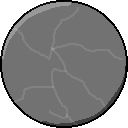
\includegraphics{Prog2_EA_V2/Art/EndTurnHover.png}\end{center}
	\subsection{EndTurnIdle}
	\begin{center}
\includegraphics{Prog2_EA_V2/Art/EndTurnIdle.png}\end{center}
	\subsection{EndTurnPressed}
	\begin{center}
\includegraphics{Prog2_EA_V2/Art/EndTurnPressed.png}\end{center}
	\subsection{Flux}
	\begin{center}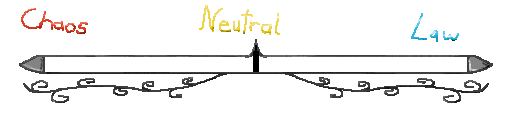
\includegraphics{Prog2_EA_V2/Art/Flux.png}\end{center}
	\subsection{Frame\_Player\_Lime}
	\begin{center}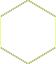
\includegraphics{Prog2_EA_V2/Art/Frame_Player_Lime.png}\end{center}
	\subsection{Frame\_Player\_Red}
	\begin{center}
\includegraphics{Prog2_EA_V2/Art/Frame_Player_Red.png}\end{center}
	\subsection{Frame\_Player\_Yellow}
	\begin{center}
\includegraphics{Prog2_EA_V2/Art/Frame_Player_Yellow.png}\end{center}
	\subsection{GameBackground}
	\begin{center}
\includegraphics[width=\textwidth
		]{Prog2_EA_V2/Art/GameBackground.jpg}\end{center}
	\subsection{Giant}
	\begin{center}
\includegraphics{Prog2_EA_V2/Art/Giant.png}\end{center}
	\subsection{Hellhound}
	\begin{center}\includegraphics{Prog2_EA_V2/Art/Hellhound.png}\end{center}
	\subsection{Hex\_Frame}
	\begin{center}\includegraphics{Prog2_EA_V2/Art/Hex_Frame.png}\end{center}
	\subsection{Hex\_Frame\_Highlighted\_atk}
	\begin{center}\includegraphics{Prog2_EA_V2/Art/Hex_Frame_Highlighted_atk.png}\end{center}
	\subsection{Hex\_Frame\_Highlighted\_atk\_move}
	\begin{center}\includegraphics{Prog2_EA_V2/Art/Hex_Frame_Highlighted_atk_move.png}\end{center}
	\subsection{Hex\_Frame\_Highlighted\_move}
	\begin{center}\includegraphics{Prog2_EA_V2/Art/Hex_Frame_Highlighted_move.png}\end{center}
	\subsection{Hex\_Frame\_Selected}
	\begin{center}\includegraphics{Prog2_EA_V2/Art/Hex_Frame_Selected.png}\end{center}
	\subsection{Hex\_Height\_0}
	\begin{center}\includegraphics{Prog2_EA_V2/Art/Hex_Height_0.png}\end{center}
	\subsection{Hex\_Height\_1}
	\begin{center}\includegraphics{Prog2_EA_V2/Art/Hex_Height_1.png}\end{center}
	\subsection{Hex\_Height\_2}
	\begin{center}\includegraphics{Prog2_EA_V2/Art/Hex_Height_2.png}\end{center}
	\subsection{Hex\_Height\_3}
	\begin{center}\includegraphics{Prog2_EA_V2/Art/Hex_Height_3.png}\end{center}
	\subsection{Hit}
	\begin{center}\includegraphics{Prog2_EA_V2/Art/Hit.png}\end{center}
	\subsection{Hydra}
	\begin{center}\includegraphics{Prog2_EA_V2/Art/Hydra.png}\end{center}
	\subsection{IcarusTower}
	\begin{center}\includegraphics{Prog2_EA_V2/Art/IcarusTower.png}\end{center}
	\subsection{MagicBolt}
	\begin{center}\includegraphics{Prog2_EA_V2/Art/MagicBolt.png}\end{center}
	\subsection{ManaBar}
	\begin{center}\includegraphics{Prog2_EA_V2/Art/ManaBar.png}\end{center}
	\subsection{ManaCost}
	\begin{center}\includegraphics{Prog2_EA_V2/Art/ManaCost.png}\end{center}
	\subsection{Mana\_Crystal}
	\begin{center}\includegraphics{Prog2_EA_V2/Art/Mana_Crystal.png}\end{center}
	\subsection{Manticore}
	\begin{center}\includegraphics{Prog2_EA_V2/Art/Manticore.png}\end{center}
	\subsection{MenuBackground0}
	\begin{center}\includegraphics{Prog2_EA_V2/Art/MenuBackground0.png}\end{center}
	\subsection{MenuBackground1}
	\begin{center}\includegraphics{Prog2_EA_V2/Art/MenuBackground1.png}\end{center}
	\subsection{MenuBackground2}
	\begin{center}\includegraphics{Prog2_EA_V2/Art/MenuBackground2.png}\end{center}
	\subsection{MenuBackground3}
	\begin{center}\includegraphics{Prog2_EA_V2/Art/MenuBackground3.png}\end{center}
	\subsection{NoImage}
	\begin{center}\includegraphics{Prog2_EA_V2/Art/NoImage.png}\end{center}
	\subsection{Obstacle}
	\begin{center}\includegraphics{Prog2_EA_V2/Art/Obstacle.png}\end{center}
	\subsection{Paladin}
	\begin{center}\includegraphics{Prog2_EA_V2/Art/Paladin.png}\end{center}
	\subsection{Pegasus}
	\begin{center}\includegraphics{Prog2_EA_V2/Art/Pegasus.png}\end{center}
	\subsection{PlayerCharacter\_Wizard\_lime}
	\begin{center}\includegraphics{Prog2_EA_V2/Art/PlayerCharacter_Wizard_lime.png}\end{center}
	\subsection{PlayerCharacter\_Wizard\_purple}
	\begin{center}\includegraphics{Prog2_EA_V2/Art/PlayerCharacter_Wizard_purple.png}\end{center}
	\subsection{PlayerCharacter\_Wizard\_red}
	\begin{center}\includegraphics{Prog2_EA_V2/Art/PlayerCharacter_Wizard_red.png}\end{center}
	\subsection{PlayerCharacter\_Wizard\_yellow}
	\begin{center}\includegraphics{Prog2_EA_V2/Art/PlayerCharacter_Wizard_yellow.png}\end{center}
	\subsection{RandomWand}
	\begin{center}\includegraphics{Prog2_EA_V2/Art/RandomWand.png}\end{center}
	\subsection{SapphireDragon}
	\begin{center}\includegraphics{Prog2_EA_V2/Art/SapphireDragon.png}\end{center}
	\subsection{Skeleton}
	\begin{center}\includegraphics{Prog2_EA_V2/Art/Skeleton.png}\end{center}
	\subsection{Summon}
	\begin{center}\includegraphics{Prog2_EA_V2/Art/Summon.png}\end{center}
	\subsection{Lion}
	\begin{center}\includegraphics{Prog2_EA_V2/Art/SummonableCreature_Lion.png}\end{center}
	\subsection{UndeadWand}
	\begin{center}\includegraphics{Prog2_EA_V2/Art/UndeadWand.png}\end{center}
	\subsection{Vampire}
	\begin{center}\includegraphics{Prog2_EA_V2/Art/Vampire.png}\end{center}
	\subsection{Vengeance}
	\begin{center}\includegraphics{Prog2_EA_V2/Art/Vengeance.png}\end{center}
	\subsection{Windwalker}
	\begin{center}\includegraphics{Prog2_EA_V2/Art/Windwalker.png}\end{center}
	\subsection{Zombie}
	\begin{center}\includegraphics{Prog2_EA_V2/Art/Zombie.png}\end{center}
	%
\end{document}
%Inhalt End
%
%
%
%
%
%
%
%